

%
%  PhD Dissertation 
%
%  Created by Fortin, Daniel C
%
\documentclass[12pt]{isuthesis}

%%%%%%%%%%%%%%%%%%%
%  packages                      
%%%%%%%%%%%%%%%%%%%
% Standard, old-style thesis
\usepackage{isutraditional} 
\chaptertitle

% Old-style, thesis numbering down to subsubsection
\alternate 
\usepackage{rotating}

\usepackage{booktabs}

% Bibtex related stuff
\usepackage{natbib} 
\bibliographystyle{apa} \bibpunct{(}{)}{;}{a}{}{,}

% mathematical symbols
\usepackage{amsmath, amssymb} 
\usepackage{stackrel} 
\usepackage{arydshln}

% set graphics path(s). Latex will search for graphics in these directories
\graphicspath{
	{/Users/dan410/Google Drive/Research/Write_ups/Dissertation/Images-nonparametric/sim-study/} 	{/Users/fort002/Google Drive/Research/Projects/SimStudy_weighted_cov_est/Plots/}
} 

% graphics packages
%\usepackage[pdftex]{graphicx}
\usepackage{caption} 
\usepackage{subcaption}

%\usepackage{pdfpages}
% formating tables
\usepackage{multirow}

%Optional Package to add PDF bookmarks and hypertext links
\usepackage[pdftex,hypertexnames=false,linktocpage=true]{hyperref} \hypersetup{colorlinks=true,linkcolor=blue,anchorcolor=blue,citecolor=blue,filecolor=blue,urlcolor=blue,bookmarksnumbered=true,pdfview=FitB}

% optional package to sync pdf output
%\usepackage{pdfsync}
% optional package to create highlighted notes within the document indicating work that needs to be done
\usepackage{todonotes} 
\usepackage{lineno}
\usepackage{xcolor, colortbl}
\newcommand{\mc}[2]{\multicolumn{#1}{c}{#2}}
\definecolor{Gray}{gray}{0.85}
\definecolor{LightCyan}{rgb}{0.88,1,1}
\definecolor{lightgray}{gray}{0.9}

\newcolumntype{a}{>{\columncolor{Gray}}c}
\newcolumntype{b}{>{\columncolor{white}}c}

%\linenumbers
% theorem environments
\usepackage{amsthm} 
\newtheorem{thm}{Theorem}[section] 
\newtheorem{lemma}{Lemma}[section]

%%%%%%%%%%%%%%%%%%%%%%%%%%%%%%%%%%%%%%%%%%%
%  list of user-defined commands         
%%%%%%%%%%%%%%%%%%%%%%%%%%%%%%%%%%%%%%%%%%%
\renewcommand{\L}{\mathcal{L}} 
\renewcommand{\S}{\mathcal{S}} 
\renewcommand{\P}{\mathcal{P}} 
\newcommand{\A}{\mathcal{A}} 
\newcommand{\C}{\mathcal{C}} 
\newcommand{\X}{\mathcal{X}} 
\newcommand{\Y}{\mathcal{Y}} 
\newcommand{\T}{\mathcal{T}} 
\newcommand{\N}{\mathcal{N}} 
\newcommand{\Tmat}{\mathbf{T}} 
\newcommand{\Rmat}{\mathbf{R}}

%\renewcommand{\H}{\ensuremath{\mathcal{H}}}
\newcommand{\R}[1]{\ensuremath{ R_{#1} }}

%\newcommand{\RR}[2]{\ensuremath{ R_{#1<#2>} }}
\renewcommand{\H}{\mathcal{H}}

%\newcommand{\HH}[2]{\ensuremath{ R_{#1<#2>} }}
\newcommand{\tsum}{\ensuremath{\oplus}} 
\newcommand{\tprod}{\ensuremath{\otimes}} 
\newcommand{\tminus}{\ensuremath{\ominus}} 
\newcommand{\Real}{\ensuremath{ \mathbb{R} }} 
\newcommand{\norm}[1]{\left\|#1\right\|} 
\newcommand{\bbeta}{\boldsymbol\beta} 
\newcommand{\balpha}{\boldsymbol\alpha} 
\newcommand{\bgamma}{\boldsymbol\gamma} 
\newcommand{\bepsilon}{\boldsymbol\epsilon} 
\newcommand{\blambda}{\boldsymbol\lambda} 
\newcommand{\wh}[1]{\widehat{#1}} 
\newcommand{\inner}[2]{\langle #1, #2 \rangle}
\renewcommand{\balpha}{\boldsymbol\alpha}

\newcommand{\hk}{H(K)} 
\newcommand{\hkk}{H(K\otimes K)}

%%%%%%%%%%%%%%%%%%%%%%%%%
%  Begin Document                      
%%%%%%%%%%%%%%%%%%%%%%%%%
\begin{document}

\DeclareGraphicsExtensions{.jpg, .pdf, .png, .mps}

%%% Title Page %%%
%!TEX root = ../dissertation.tex

% Template Titlepage File
\title{Statistical models for spatially indexed functional data}
\author{Daniel Clayton Fortin}
\major{Statistics}
\degree{DOCTOR OF PHILOSOPHY}
\level{doctorate}
\mprofs{Petru\c{t}a Caragea}{Zhengyuan Zhu}
\committee{3}
\members{Heike Hofmann \\ Dan Nordman \\ Stephen Vardeman}
\notice
% Add these additional lines for a Doctoral Dissertation
%\level{doctoral}
%\format{dissertation}
%\committee{4}
%\members{Mary Jones \\ Bjork Petersen \\ Sam Anders \\ Harold Jones}
% Add these additional lines for a Creative Component
% - also comment out the \maketitle command
%\format{Creative Component}
%\submit{the graduate faculty}
\maketitle


%%% Optional thesis dedication
\chapter*{DEDICATION}

Put dedication here

%I would like to dedicate this thesis to my wife Glenda and
%to my daughter Alice without whose support I would not have
%been able to complete this work.
%I would also like to thank my friends and family for their loving guidance and
%financial assistance during the writing of this work.



%%% Preface Content %%%
\pdfbookmark[1]{TABLE OF CONTENTS}{table}
\tableofcontents \addtocontents{toc}{
\def\protect\@chapapp{}} \cleardoublepage \phantomsection \addcontentsline{toc}{chapter}{LIST OF TABLES}

\listoftables
\cleardoublepage \phantomsection \addcontentsline{toc}{chapter}{LIST OF FIGURES}
\listoffigures

%%% Comment out the next line if NOT using chaptertitle
\addtocontents{toc}{
\def\protect\@chapapp{CHAPTER\ }}

%%% Optional Acknowledgements
\cleardoublepage \phantomsection

\specialchapt{ACKNOWLEDGEMENTS}
%!TEX root = ../dissertation.tex
A great deal of thanks is due to my major professors, Dr. Petru\c{t}a Caragea and Dr. Zhengyuan Zhu, for their guidance, insights, and dedication throughout the research and dissertation writing process. I would also like to thank my committee members for their advice and support: Dr. Heike Hofmann, Dr. Dan Nordman, and Dr. Stephen Vardeman. In particular, I would like to thank Dr. Stephen Vardeman for the many enjoyable conversations we have had over the past few years including advice on academic life, efficient grocery shopping, and the nuances of reproducing kernel Hilbert spaces. 

I would also like to thank my friends in the statistics department and my family for their friendship and countless caffein-fueled conversations that helped me stay motivated throughout this journey. 



%%% Optional thesis abstract
%\cleardoublepage \phantomsection
%\specialchapt{ABSTRACT}

This is the text of my abstract that is part of the thesis itself.
The abstract describes the work in general and the heading and style
match the rest of the document.


\newpage 
\pagenumbering{arabic}

%%% Body %%%
%!TEX root = ../dissertation.tex

\chapter{INTRODUCTION}
%\begin{spacing}{1.9}
In many instances, it is useful to view data as a collection of curves. The study of human growth is a common example used to motivate this view, where data arising from the study can be viewed as collection of individual growth curves.  The second derivative of the growth curves are used to study growth acceleration and identify common growth spurts. In studies like this, where the questions motivating the analysis relate to properties of curves, it makes sense to view the fundamental datum as a curve and refer to the collection of curves as \emph{functional data}.  %Ferraty and Vieu (2006) characterize this by defining a functional random variable as one which takes values in an infinite dimensional space. 

The publication of the book \emph{Functional Data Analysis}, the seminal work by \cite{FDA}, inspired substantial interest in developing statistical models for functional data.  Though their book describes the extension of linear models to the functional setting, it stops short of allowing for complex dependence structures by assuming independence between observed curves. For curves observed in space, this assumption is often violated. Examples of functional data which have a spatial index are becoming more common in scientific studies: data collected by weather stations, oceanology measurements taken by seals equipped with sensor devices, peak electron density measurements collected by ionosonde stations in the northern hemisphere, and satellite measurements of environmental variables. Therefore,  research on functional models for spatial data is a very important and actual topic.

%  In environmental data,  the correlations exhibited between observations in space may be of scientific interest and often the primary goal of the analysis is prediction of a environmental variable at an unobserved location.  In this setting, geostatistical models are often used. The extension of geostatistical models for functional data were first considered by \cite{Goulard:1993}, who proposed two possible approaches: one approach involves cokriging by reducing the functional response to a multivariate response, while the other approach untilizes a functional version of the variogram.  The functional variogram approach has been further developed by \cite{Giraldo:2010jx} and \cite{Nerini:2010ba}. 

%Examples of spatially indexed functional data have also been considered for functional data with a multilevel structure, often arising in the case of designed experiments. In these cases, a mixed model framework is typically used and much work has been done extending mixed model methodology to accommodate functional observations (\cite{Li:2007dn}, \cite{Morris:2006wq},\cite{Di:2009dz}, \cite{Baladandayuthapani2008},\cite{Staicu:2010ez}, \cite{Scheipl:2012tm}). 

When data are random curves rather than scalars or vectors, it is necessary to have a convenient way to represent the curves.  A standard approach is to express the curves in terms of a known basis set (e.g. b-spline, wavelets, Fourier). An alternative, and what we believe to be a more attractive choice for spatial functional data, is an empirical basis consisting of functional principal components (FPC). When curves are represented by a linear combination of basis functions, the variation among curves can be investigated through the variation among the coefficients of the basis functions. Thus, spatial similarity between curves can be modeled through the correlation structure associated with the basis function coefficients viewed as scalar random fields. Using a finite basis representation of the curves, each curve is identified by its vector of coefficients, allowing the use of multivariate methods; moreover, it is well known that principal components achieve maximum efficiency in terms of representing variation in the data for a fixed dimension. 

%To clarify what is meant by functional principal components, here is a brief review of the relevant mathematical results.  
%
%A process $X(t)$, defined on a closed interval $\T  \subset \Real$,  with finite covariance possesses a sequence of orthonormal eigenfunctions $\{\psi_m(t)\}_{m=1,2,\ldots}$, which form a complete bases of the functional space, with associated nonnegative and nondecreasing eigenvalues $\{\lambda_m \}_{m=1,2,\ldots}$. By the Karhunen-Loeve expansion, the process $X(t)$ admits the representation
%\begin{equation*}
%X(t) =  \sum_{m=1}^{\infty}\alpha_m \psi_m(t), \mbox{ where  } \alpha_m = \int_{\T} X(t) \psi_m(t)dt.
%\end{equation*}
%
%The random variables $\{\alpha_m \}_{m=1,2,\ldots}$ are the functional principal component scores of $X(t)$, which are uncorrelated and satisfy $E(\alpha_m)=0$ and var($\alpha_m$) = $\lambda_m$, $\sum_m \lambda_m < \infty$.\\
%Remarks:
%\begin{enumerate}
%	\item The eigenfunctions are orthonormal in the space $L^2[\T]$ and the FPC scores are uncorrelated random variables.
%	\item The eigenfunctions efficiently capture the dominant modes of variation in the observed curves.
%	\item The eigenvalues often decrease rapidly and thus the infinite dimensional process $X(t)$ can be well approximated by a small number of FPCs. 
%\end{enumerate}

%This framework is often adopted (e.g., \cite{Yao:2005cv}, \cite{Gromenko2012}, \cite{Di:2009dz}); however, 
This approach introduces the non-trivial problem of estimating the principal component functions from observed data. Estimation of principal component functions can be accomplished by estimating the covariance function through bivariate smoothing and then computing the eigenfunctions of the estimated covariance surface (some alternative methods are described in \cite{FDA} Ch. 8 and Ch. 9). Because of this, much effort has been devoted to methods for nonparametric covariance estimation and eigenfunction estimation ( \cite{Yao:2005cv}, \cite{Li:2007dn}, \cite{Cai:2010vr}).  Of the literature on nonparametric covariance function estimation, \cite{Cai:2010vr} provides the most general framework by assuming curves belong to a reproducing kernel Hilbert space (RKHS) and utilizing theoretical results developed for spline smoothing methods. This framework allows for closed form estimation of the eigenfunctions and their derivatives, so one does not need to discretize the covariance function and approximate eigenfunctions with eigenvectors.  This is particularly useful because we use eigenfunctions as a basis set for further model building and not just as an exploratory tool. 

In this dissertation we work in a reproducing kernel Hilbert space framework, representing curves with a principal component function basis, and model spatial dependence between curves through FPC scores.  
\begin{itemize}
\item In Chapter \ref{ch:covariance estimation} we describe an estimator for principal component functions by extending the methods developed in \cite{Cai:2010vr}. We have developed an R implementation of this method. In our implementation one can easily produce list object containing the estimated principal component functions. We have also developed an empirical basis specification  within the fda package framework, so that the estimated principal component functions can be used as a basis object.  %Ramsay and Silverman have stated that a future fda release will contain support for empirical bases, but I do not believe this has been implemented yet. 
\item In Chapter \ref{ch:functional kriging} we describe how this framework can be used for ordinary kriging prediction for functional data. We also describe our current work on improving the nonparametric covariance estimator by incorporating spatial dependence in the estimation of the covariance function. 
\item  In Chapter \ref{future work} we discuss future directions in model development motivated by spatial functional data arising from a phenological study in India. Some of the scientific questions related to these data involve identifying biological life-cycles, which can be cast in terms of derivatives of the curves (e.g., global mixima, inflection points). This fact further motivates the functional data approach, as it is a natural way in which one can estimate and represent derivatives. 
\item In Appendix \ref{ch:theoretical background} I have included some of the theoretical background necessary to understand the developments in Chapter \ref{ch:covariance estimation}. There is no original work in this chapter and it only serves to make this document a little more self-contained. 
\end{itemize}

Plans for future work to complete the dissertation are described in the last section of the respective chapters. 

%
%In functional data analysis a datum is considered to be a function defined on a domain $\T$ and a data set consists of a collection of functions.  The collection of curves can be conceptualized as realizations from a stochastic process. In practice each curve is observed at finitely many points and with noise, thus a regularization procedure --- converting raw data to smooth curves --- is typically an initial step. A popular regularization approach involves expressing the curves in terms of a finite basis (e.g. Fourier, wavelet, b-spline). An attractive alternative is an empirical basis consisting of principal component functions. Principal component functions are the infinite dimensional version of principal component vectors in that they define a coordinate system aligned with the major modes of variability within the data. Deriving principal component functions---similarly to deriving principal component vectors---involves an eigen-analysis of the covariance operator.  
%
%In functional data analysis the covariance operator is not a matrix, but a bivariate function defined on a rectangle. Eigen-analysis of a bivariate function is not as straightforward as it matrix counterpart, but we adopt a method proposed by \cite{Cai2010} who, by working in a reproducing kernel Hilbert space framework, give formulas for closed form estimates of the eigenfunctions. In their method, covariance function estimation is approached as a bivariate smoothing problem. Assuming the curves belong to a RKHS naturally identifies the covariance function as belonging the the tensor product reproducing kernel Hilbert space. The estimator of the covariance function is cast as a penalized regression problem utilizing the norm on the tensor product space. It is has been shown that the estimator has a finite dimensional representation, reducing the eigenfunction problem to an eigenvector problem.

%\end{spacing}



%!TEX root = ../dissertation.tex
\chapter{NONPARAMETRIC COVARIANCE FUNCTION AND PRINCIPAL COMPONENT FUNCTION ESTIMATION FOR FUNCTIONAL DATA} \label{ch:covariance estimation}

\section{Abstract} 

% (fold)
\label{sec:abstract}

Functional principal components has gained much popularity in the are of functional data analysis as an exploratory and as a modeling tool. Principal compenent functions are known to correspond to the eigenfunctions of the covariance operator. Due to this fact, much work has been done on flexible methods for covariance function estimation. In this paper we investigate an approach to covariance function estimation where the curves are assumed to belong to a reproducing kernel Hilbert space (RKHS). By assuming curves belong to a RKHS, it has been shown that the covariance function necessarily belongs to the corresponding tensor product space--which is itself an RKHS. This fact motivates an approach for nonparametric estimation using the norm on the tensor product space as a smoothing penalty. We adopt this framework and explore how the choice of function space and penalty effect the representation of the estimator---in particular we consider function spaces where the norm is defined on a subspace, resulting in a non-empty unpenalized subspace. We describe the form of the covariance function estimator in this case and derive closed form estimators of the principal component functions. 

% section abstract (end)
\section{Introduction} 

% (fold)
\label{sec:introduction}

Functional principal components are often used in functional data analysis as an efficient way to represent curves. In multivariate methods, principal components can be derived through an eigen-decomposition of the covariance matrix; however, with functional data the covariance is not a matrix, but a continuous bivariate function. When the number of observations per curve is sparse often one approaches the problem by pooling covariance information from each curve and performing bivariate smoothing. What seems most common in the literature is to use local polynomial smoothing (\cite{Yao:2005cv}). \cite{Cai:2010vr} propose a framework for nonparametric covariance function estimation motivated by theory for smoothing splines, which make use properties of reproducing kernel Hilbert space (RKHS). One major benefit of this approach is that it can be used for both sparse and dense functional data, whereas previous methods have been shown to work well in one case but not optimal in the other. The field of functional data analysis is relatively new, growing, and in flux. Unifying theoretical results serve to strengthen the foundation of the field and provide much needed insight. The theoretical framework of RKHS seems particularly suited for the task of covariance function estimation as the rate of convergence can be shown to be near-optimal. A more practical benefit of this approach is the ability to derive closed form estimates of the eigenfunctions. This fact alone makes this appraoch extremely useful, as one often seeks to represent curves using a principal component function basis. In this work, we adopt and investigate this approach to covariance function estimation gaining insight into Hilbert space decompositions as they relate to specific reproducing kernels that are used by practioners; derive a more general version of the eigenfunction estimator; and provide a computational tool in the form of an R package including functions for both covariance function estimation and principal component function estimation (https://github.com/dan410/sseigfun).

For curves belonging to a RKHS, it can be shown that the covariance function resides in the tensor product reproducing kernel Hilbert space $\H\otimes \H$. The tensor product space is itself a RKHS whose reproducing kernel is strait forward to derive for the reproducing kernel on $\H$. Based on this result, a natural regularization procedure for covariance function estimation is the following: 
\begin{equation}
	\label{eq:cy-cov-est} \hat{C}_{\lambda} = \stackrel[C \in \H\otimes\H]{}{\mbox{argmin}} \{l_{n}(C)+\lambda\left\Vert C\right\Vert _{\H\otimes \H}^{2}\}, 
\end{equation}
where

%\begin{equation}
%l_{n}(C)=\frac{1}{n*}\sum_{i=1}^{n}\sum_{1\leq j_{1}\neq j_{2}\leq m}([Y_{ij_{1}}-\mu_{0}(t_{ij})][Y_{ij_{2}}-\mu_{0}(t_{ij_{2}})]-C(t_{ij_{1}},t_{ij_{2}}))^{2}
%\label{eq:loss}
%\end{equation}
% where $n* = 1/nm(m-1)$ and
$\lambda\geq0$ is a tuning parameter that balances the fidelity to the data measured by $l_{n}$ and smoothness of the estimate measured by the squared RKHS norm.

In \cite{Cai:2010vr} the convergence rate of this estimator was shown to be superior to the optimal rate for general bivariate smoothing on $[0,1]\times[0,1]$, which is attributed to the fact that estimation is performed over functions in $\H \tprod \H$ instead of the typical Sobelev space used for bivariate smoothing. This implies that the tensor product RKHS is to a certain degree smaller than the typical Sobelev space, thus reducing the effect of ``the curse of dimensionality''.

Using standard arguments from smoothing spline theory (see \cite{Wahba:1990}), the covariance function estimator \eqref{eq:cy-cov-est} has a finite dimensional representation. Further, using this representation, closed form expressions for the eigenfunctions can be derived. This is a significant benefit, as one often has to numerically approximate the eigenfunctions by discretizing the covariance function.

This approach assumes that the reproducing kernel is known and that the tensor product norm corresponding to the reproducing kernel penalizes smoothness in an appropriate way. It seems important, from a practical point of view, to have a clear understanding of how the penalty functional is operating. To accomplish this we propose an approach that begins with defining how univariate functions are penalized on the marginal domain (typically done by defining an appropriate high order derivative), then use the implied penalty on the tensor product domain to estimate the covariance function. This approach is more attractive from a practitioner's point of view, because it is more natural to define a differential operator to penalize smoothness, and in this case the functions annihilated by the differential operator form a non-null subspace. \cite{Cai:2010vr} proposes, as an example, a kernel based on penalizing the integrated squared second derivative, but define a function space where all non-zero functions are penalized. It is not clear if this function space was chosen other than for mathematical convenience as it has a trivial unpenalized subspace. We show how the estimator can be generalized to allow for non-trivial unpenalized spaces. 

Our approach allows for the typical function space, 
\begin{equation}
	W_2 = \{f : f, f' \mbox{ absolutely continuous}, f'' \in L_2[0,1]\},
\end{equation} 
to be used and accounts for the decomposition of the function space into penalized and unpenalized subspaces. To illustrate this, recall the general development for the smoothing spline in the univariate case (\cite{Wahba:1990}): The solution of 
\begin{equation}
	\widehat{f}_{\lambda} = \hspace{.07in}\stackrel[f \in \H]{}{\mbox{argmin}} \left\{ \frac{1}{n}\sum_{i=1}^{n}(y_i - f(t_i))^2 + \lambda\norm{f}^2_{\H} \right\} 
\end{equation}
has the form 
\begin{equation}
	\hat{f}(t) = \sum_{i=1}^N c_iR(t, t_i), 
\end{equation}
while the solution of 
\begin{equation}
	\widehat{f}_{\lambda} = \hspace{.07in}\stackrel[f \in \H]{}{\mbox{argmin}} \left\{ \frac{1}{n}\sum_{i=1}^{n}(y_i - f(t_i))^2 + \lambda\norm{P_1(f)}^2_{\H_1} \right\} \label{eq:unpenalized objective function} 
\end{equation}
has the form 
\begin{equation}
	\hat{f}(t) = \sum_{j=1}^M d_j\phi_j(t) + \sum_{i=1}^N c_iR_1(t, t_i), \label{eq:unpenalized solution} 
\end{equation}
where $\{\phi_j(\cdot)\}_{j=1}^M$ are a basis for the space of unpenalized functions $\H_0$ and $P_1(f)=f_1$ is the projection of $f$ onto the space $\H_1$. (Details of the derivation of \eqref{eq:unpenalized solution} from \eqref{eq:unpenalized objective function} are shown in the Appendix ). In Section \ref{sec:covariance_function_estimation} we show how the regularization procedure for covariance function can account for this type of decomposition. In Section \ref{sec:estimation_of_functional_principal_components} we derive closed form estimators of the principal component functions based on the generalized covariance estimator.

% section introduction (end)
\section{Methodology} 

% (fold)
\label{sec:methodology}

In the following we assume $\T$ to be the interval $[0,1]$. Let $X(\cdot)$ be a second order stochastic process with covariance function
\[ C_{0}(s,t)=E([X(s)-E(X(s))][X(t)-E(X(t))]),\mbox{ }\forall s,t\in \T. \]
Further, assume $X(\cdot)$ takes values in a reproducing kernel Hilbert space $\H$ with corresponding reproducing kernel $R(s,t)$. The reproducing kernel $R(s,t)$ has the property $\inner{f(s)}{R_t(s)}_{\H} = f(t)$ for all $f \in \H$, where $R_t(s)$ is notation for $R(s,t)$ holding the second coordinate fixed. The function $R_t(s)$ belongs to $\H$; as an immediate consequence of the reproducing property $\inner{R_{t_1}(s)}{R_{t_2}(s)} = R(t_1, t_2)$. 

%Note that this is a key property, since it shows that inner products involving the reproducing kernel function are equivalent to function evaluation.  
Let $\{X_{1},X_{2},\dots,X_{N}\}$ be a collection of independent realizations of $X$, and we consider the following observation model
\[ Y_{ij}=X_{i}(t_{ij})+\epsilon_{ij},\mbox{ }j=1,\dots,m;\mbox{ }i=1,\dots,N, \]
where the sampling locations are independently drawn from a common distribution on $\T,$ and $\epsilon_{ij}$ are independently and identically distributed measurement errors with mean zero and finite variance $\sigma_{0}^{2}.$ It is further assumed that the random functions $X,$ sampling locations $t_{ij},$ and measurement errors $\epsilon$ are mutually independent. 

The development in this section relies on the fact that a closed subspace of a Hilbert space induces a natural partition of the space into a direct sum of the closed subspace and its orthogonal complement (\cite{Gu2002} gives a concise overview of the relevant Hilbert space theory). The subspace consisting of unpenalized functions is a closed subspace and it is convenient to express $\H$ as a direct sum decomposition $\H = \H_0 \oplus \H_1$, where on $\H_1$ the penalty functional is a full squared norm and $\H_0$ consists of functions in $\H$ which will not be penalized. With this orthogonal decomposition, any function $f \in \H$ has the representation $f = f_0 + f_1$, where $f_0 \in \H_0$ and $f_1 \in \H_1$. It is well known that the reproducing kernel $R$ on $\H$ can be expressed as $R = R_0 + R_1$, where $R_0$ is the reproducing kernel on $\H_0$ and $R_1$ is the reproducing kernel on $\H_1$.

Covariance function estimation takes place on the product domain $\T_1\times \T_2$ = $[0,1]\times[0,1]$. Denote by $\H_{<1>}$ and $\H_{<2>}$ the reproducing kernel Hilbert space on $\T_1$ and $\T_2$, respectively. Let $\H_{<1>}=\H_{0<1>} \oplus\H_{1<1>}$ and $\H_{<2>} = \H_{0<2>} \oplus \H_{1<2>}$ be the direct sum decomposition of spaces on the marginal domains into their unpenalized and penalized subspaces. Using these decompositions, the tensor product space $\H_{<1>} \otimes \H_{<2>}$ has the representation 
\begin{equation*}
	\H_{<1>} \otimes \H_{<2>} =( \H_{0<1>} \oplus \H_{1<1>}) \otimes (\H_{0<2>} \oplus \H_{1<2>}) 
\end{equation*}
which can be expanded into the following tensor sum 
\begin{equation}
	\H_{<1>} \otimes \H_{<2>} = ( \H_{0<1>} \otimes\H_{0<2>}) \oplus (\H_{0<1>} \otimes \H_{1<2>}) \oplus ( \H_{1<1>} \otimes \H_{0<2>}) \oplus (\H_{1<1>} \otimes \H_{1<2>}). \label{eq:tpsum} 
\end{equation}
Equation \eqref{eq:tpsum} is a direct sum of tensor product reproducing kernel Hilbert spaces, where the subspace corresponding to $ \H_{0<1>} \otimes\H_{0<2>}$ consists only of unpenalized functions. As in the univariate case, the solution to the penalized smoothing problem when unpenalized subspaces are allowed will involve linear combination of the basis functions for the unpenalized subspace. 

The main goal in what follows is to describe the form of the covariance function estimator when the tensor product space has a decomposition as in \eqref{eq:tpsum}. We describe the form of the estimator in this case as well as derive the principle component functions. Since our focus is on practical implementation of this method, we focus on the most common case where the smoothing penalty on the marginal domain is given by the integral of the squared second derivative.

% section methodology (end)
\section{Covariance function estimation} 

% (fold)
\label{sec:covariance_function_estimation}

Consider the space $\H = \{f : f, f' \mbox{ absolutely continuous}, f'' \in L_2[0,1]\}$. On this space the term $\int_0^1 f''g''dx$ is a semi-inner-product which can be extended to a full inner product by defining an inner product on the subspace $\H_0 = \{f : f'' = 0\}$. Common choices for inner products in $\H_0$ are $\inner{f}{g}_0 = f(0)g(0) + f'(0)g'(0)$ or $\inner{f}{g}_0 = (\int_0^1fdx)(\int_0^1gdx) + (\int_0^1f'dx)(\int_0^1g'dx)$. We work with the latter because it corresponds to a mathematically convenient expression for the reproducing kernel. 

The space $\H$ with inner product 
\begin{align*}
	\inner{f}{g} &= \inner{f}{g}_0 + \inner{f}{g}_1 \\
	&= \left(\int_0^1fdx\right)\left(\int_0^1gdx\right) + \left(\int_0^1f'dx\right)\left(\int_0^1g'dx\right) + \int_0^1 f''g''dx 
\end{align*}
is a RKHS with a reproducing kernel that can be conveniently expressed in terms of the functions 
\begin{equation}
	k_r(x) = -\left( \sum_{\mu = -\infty}^{-1} + \sum_{\mu=1}^{\infty} \right) \frac{\exp(2\pi i \mu x)}{(2 \pi i \mu)^r}, r = 1,2, \dots. \label{eq:kfuns} 
\end{equation}
The functions $k_r(x)$ in \eqref{eq:kfuns} are scaled Bernoulli polynomials, $k_r(x) = \frac{B(r)}{r!}$. The space $\H$ has an orthogonal decomposition $\H = \H_0 \tsum \H_1$ with corresponding reproducing kernel $R(x,y) = R_0(x,y) + R_1(x,y)$, where 
\begin{align}
	R_0(x,y) &= 1 + k_1(x)k_1(y) \\
	R_1(x,y) &= k_2(x)k_2(y) - k_4(x-y). 
\end{align}
Note that the functions $k_r(x)$ in \eqref{eq:kfuns} have a rather simple form 
\begin{align*}
	k_1(x) &= x - 0.5\\
	k_2(x) &= \frac{1}{2}(k_1^2(x) - \frac{1}{12}) \\
	k_4(x) &= \frac{1}{24} \left(k_1^4(x) - \frac{k_1^2(x)}{2} + \frac{7}{240} \right) 
\end{align*}
for $x \in [0,1]$. 

The unpenalized space $\H_0$ can be decomposed further as $\H_0 = \H_{00} \tsum \H_{01}$ with reproducing kernels 
\begin{align*}
	R_{00}(x,y) &= 1\\
	R_{01}(x,y) &= k_1(x)k_1(y).\\
\end{align*}
This formulation provides a decomposition of the unpenalized space into functions spanned by a constant and functions spanned by a linear term. This construction results in the overall decomposition $\H= \H_{00} \tsum \H_{01} \tsum \H_1$. Using this decomposition of $\H$ on both marginal domains of $[0,1] \times [0,1]$ results in a natural decomposition of the tensor product space
\[ \H_{<1>} \tprod \H_{<2>} = (\H_{00<1>} \tsum \H_{01<1>} \tsum \H_{1<1>})\tprod (\H_{00<2>} \tsum \H_{01<2>} \tsum \H_{1<2>}) \]
into a sum of nine subspaces of the tensor product space. These nine subspaces and their corresponding reproducing kernels are shown in Table \ref{tab:tp decomp}. It is straight forward to derive the reproducing kernels in Table \ref{tab:tp decomp} using the fact that the reproducing kernel on the tensor product space is the product of the reproducing kernels on the marginal spaces, i.e. $R((x_{<1>}, x_{<2>}), (y_{<1>}, y_{<2>}) ) = R_{<1>}(x_{<1>}, y_{<1>})\times R_{<2>}(x_{<2>}, y_{<2>})$. 
\begin{table}
	[h] \centering \caption{Tensor product space decomposition with corresponding reproducing kernels.} \label{tab:tp decomp} 
	\begin{tabular}
		{|c|c|} \hline Subspace & Reproducing Kernel\tabularnewline \hline \hline $H_{00<1>}\otimes H_{00<2>}$ & 1\tabularnewline \hline $H_{00<1>}\otimes H_{01<2>}$ & $k_{1}(x_{<2>})k_{1}(y_{<2>})$\tabularnewline \hline $H_{00<1>}\otimes H_{1<2>}$ & $k_2(x_{<2>})k_2(y_{<2>}) - k_4(x_{<2>} - y_{<2>})$\tabularnewline \hline $H_{01<1>}\otimes H_{00<2>}$ & $k_1(x_{<1>})k_1(y_{<1>})$ \tabularnewline \hline $H_{01<1>}\otimes H_{01<2>}$ & $k_1(x_{<1>})k_1(y_{<1>})k_1(x_{<2>})k_1(y_{<2>})$ \tabularnewline \hline $H_{01<1>}\otimes H_{1<2>}$ & $k_1(x_{<1>})k_1(y_{<1>})[k_2(x_{<2>})k_2(y_{<2>}) - k_4(x_{<2>} - y_{<2>})]$\tabularnewline \hline $H_{1<1>}\otimes H_{00<2>}$ & $k_2(x_{<1>})k_2(y_{<1>}) - k_4(x_{<1>} - y_{<1>})$\tabularnewline \hline $H_{1<1>}\otimes H_{01<2>}$ & $[k_2(x_{<1>})k_2(y_{<1>}) - k_4(x_{<1>} - y_{<1>})]k_1(x_{<1>})k_1(y_{<1>})$\tabularnewline \hline $H_{1<1>}\otimes H_{1<2>}$ & $[k_2(x_{<1>})k_2(y_{<1>}) - k_4(x_{<1>} - y_{<1>})]\times$ \tabularnewline & $[k_2(x_{<2>})k_2(y_{<2>}) - k_4(x_{<2>} - y_{<2>})]$\tabularnewline \hline 
	\end{tabular}
\end{table}

Inspection of the tensor product subspaces listed in Table \ref{tab:tp decomp} shows that only five have the space $\H_1$ as one of their marginal domain spaces, thus it is these five spaces that comprise the space of penalized functions. In order to represent the reproducing kernel on the penalized space the following notation is useful. Denote $\H_{\nu, \mu}=\H_{\nu <1>}\otimes \H_{\mu <2>}$ and $R_{\nu, \mu}=R_{\nu <1>}R_{\mu <2>}$, then $\breve{R} = R_{1,00}+R_{1,01}+R_{00,1}+R_{01,1}+R_{1,1}$ is the reproducing kernel on $\breve{\H} = \H_{1,00}\oplus\H_{1,01}\oplus\H_{00,1}\oplus\H_{01,1}\oplus\H_{1,1}$. The space $\breve{\H}$ contains all functions on the product domain that have a non-zero smoothing penalty.

Let $\mathbf{b}^{(i)} = [(y_{ij}-\mu(t_{ij}))(y_{ij'}-\mu(t_{ij'}))]_{1\leq j\neq j'\leq m}$, $i=1, \dots, n$. Let
\[ \mathbf{b} = (\mathbf{b}^{(1)T}, \mathbf{b}^{(2)T}, \dots, \mathbf{b}^{(n)T} )^T, \]
then the vectors $\mathbf{b}^{(i)}$ contain all pairwise products of observations on the $i$th curve, excluding those that are the product of an observation with itself. We propose the following estimator:
\[ \widehat{C}_{\lambda}=\stackrel[C \in \H\otimes \H]{}{\text{ argmin}} \left\{\frac{1}{nm^2-nm} (\mathbf{b} - \mathbf{C})^T(\mathbf{b} - \mathbf{C})+\lambda\left\Vert C\right\Vert _{\breve{\H}}^{2} \right\}, \]
where

%\begin{equation}
%l_{n}(C)= (\mathbf{b} - \mathbf{C})^T(\mathbf{b} - \mathbf{C})
%\label{eq:loss1}
%\end{equation}
%and 
\[ \mathbf{C} = [C(t_{i,j}, t_{i'j'})]. \]

Using the representer theorem in \cite{Wahba:1990} theorem 1.3.1, it can be shown that the estimated covariance function has the form 
\begin{equation}
	\hat{C}(s,t) = \sum_{\nu, \mu=00,01}d_{\nu,\mu}\phi_{\nu,\mu}(s,t) + \sum_{i,j}c_{i,j}\breve{R}((t_i,t_j),(s,t))	
	%\label{eq:}
\end{equation}
The four basis functions for the unpenalized space are $\phi_{\nu,\mu}$ are $\{ 1, k_1(s), k_1(t), k_1(s)k_1(t) \}$, so the solution can be written more explicitly as 
\begin{equation}
	\hat{C}(s,t) = d_{00,00} + d_{01,00}k_1(t) + d_{00,01}k_1(s) + d_{01,01}k_1(s)k_1(t) + \sum_{i,j}c_{i,j}\breve{R}((t_i,t_j),(s,t)). \label{eq:covest} 
\end{equation}
Efficient estimation of \eqref{eq:covest} including smoothing parameter selection can be accomplished using methods described in \cite{Gu2002} and implemented in the \texttt{gss} R package. 

%\todo{include the quadratic form version of the minimization problem}
%The estimator in \eqref{eq:covest} involves slices of the reproducing kernel on the penalized space. These slices are 2-dimensional surfaces and it is of some interest to investigate these surfaces. Figure~\ref{fig:basis_fns} shows some of these functions corresponding to knot locations on a five by five grid. 
\subsection{Practical considerations for knot selection} % (fold)
\label{sub:practical_considerations_for_knot_selection}

% subsection practical_considerations_for_knot_selection (end)
In practice, when curves are not sparsely observed, the number of observed pairs $(t_i, t_j)$ will be large. In this case \cite{CFZ} recommend using knot locations forming a regular grid within the convex hull of the observed points. \cite{Kim:2004tt} investigate this with a simulation study and give a general recommendation of $10n^{2/9}$, where $n$ is the sample size on the product domain. Following this advice, we fix knot locations on a regular grid Let $t_i \in [0,1]; i=1,\dots, K$ be the chosen knot locations on the univariate domain, making $(t_i,t_j)_{1\leq i,j \leq K}$ a regular grid of knot locations on $[0,1]\times[0,1]$. The number of knot locations $K$ puts an upper bound of $K+2$ eigenfunctions because the number of knot locations plus the dimension of the unpenalized space bound the dimension of the solution space for the eigenfunctions as shown in Lemma \ref{thm:eigenfunctions}.

% section covariance_function_estimation (end)
\section{Estimation of functional principal components} 

% (fold)
\label{sec:estimation_of_functional_principal_components}

Functional principal components are related to the well-known Karhunen-Loeve representation theorem. For a square-integrable stochastic process $X(t)$ defined on a closed interval $[a,b]$, with continuous covariance $C(s,t)$, there corresponds a linear operator $[T_Cf](s) = \int_a^bC(s,t)f(t)dt$. Since $C(s,t)$ is symmetric and non-negative definite, it has the following representation 

%(see Mercer's theorem)
\begin{equation*}
	C(s,t) = \sum_{i=1}^{\infty}\lambda_i\psi_i(s)\psi_i(t), 
\end{equation*}
where $\{\psi_m(t)\}_{m=1,2,\ldots}$ are a sequence of orthonormal eigenfunctions which form a complete basis in $L_2[a,b]$, and $\{\lambda_m \}_{m=1,2,\ldots}$ are nonnegative and nondecreasing eigenvalues. In this context, an eigenfunction-eigenvalue pair $\{\lambda_j, \psi_j(t)\}$ satisfy $\int_a^bC(s,t)\psi_j(t)dt = \lambda_j\psi_j(t)$. The Karhunen-Loeve theorem states that the process $X(t)$ admits the representation 
\begin{equation*}
	X(t) = \sum_{m=1}^{\infty}\alpha_m \psi_m(t), \mbox{ where } \alpha_m = \int_a^b X(t) \psi_m(t)dt, 
\end{equation*}
and the random variables $\{\alpha_m \}_{m=1,2,\ldots}$ are uncorrelated and satisfy $E(\alpha_m)=0$ and Var($\alpha_m$) = $\lambda_m$, $\sum_m \lambda_m < \infty$. The eigenfunctions $\{\psi_m(t)\}_{m=1,2,\ldots}$ corresponding to $C(s,t)$ are called the principal component functions and the coefficients $\{\alpha_m \}$ are the functional principal component scores of $X(t)$. We seek functions $\hat{\psi}(s)$ that satisfy satisfy 
\begin{equation}
	\label{eq:eigenfuns} \int \hat{C}(s,t)\hat{\psi}(t)dt=\theta\hat{\psi}(s). 
\end{equation}

Methods for deriving principal component functions were developed in \cite{FDA} for functions represented by finite basis representation, i.e. $X(t) = \mathbf{b}'\mathbf{g}(t)$, where $\mathbf{g}(t)$ is a vector of basis functions. Using the finite dimensional covariance function representation in \eqref{eq:covest} we adapt these results by considering the vector of functions 
\begin{equation}
	\mathbf{g(\cdot)}=(1, k_1(\cdot),R_{1}(\cdot, t_1),R_{1}(\cdot, t_2),\dots, R_{1}(\cdot, t_K))'. \label{eq:g} 
\end{equation}
Using $\mathbf{g}$ in \eqref{eq:g} the covariance function estimator in \eqref{eq:covest} has the representation $\hat{C}(s,t)= \mathbf{g}(s)'A\mathbf{g}(t)$ where \vspace{0.8cm} 
\begin{center}
	$A = \left( 
	\begin{array}{cc:cccc}
		d_{00,00} & d_{01,00} & c_{1.} & c_{2.} & \dots & c_{K.}\\
		d_{00,01} & d_{01,01} & \sum_j c_{1j}k_1(t_j) & \sum_j c_{2j}k_1(t_j) & \dots & \sum_j c_{Kj}k_1(t_j)\\
		\hdashline c_{.1} & \sum_j c_{j1}k_1(t_j) & c_{11} & c_{12} & \dots & c_{1K}\\
		c_{.2} & \sum_j c_{j2}k_1(t_j) & c_{21} & c_{22} & \dots & c_{2K}\\
		\vdots & \vdots & \vdots & \vdots & \ddots & \vdots \\
		c_{.K} & \sum_j c_{jK}k_1(t_j) & c_{K1} & c_{K2} & \dots & c_{KK} 
	\end{array}
	\right)$. 
\end{center}
\vspace{0.8cm} Note that \cite{Cai:2010vr} use the tensor product norm on $\H\tprod \H$, thus there is no unpenalized subspace. In this case the matrix $A$ reduces to the bottom right submatrix. 

%Software packages, such as the gss package in R, will return the fitted coefficients $c$ and $d$ in \eqref{eq:covets}, The matrix $A$ can be constructed directly from the fitted coefficients in the output of the sspreg1() function which makes this straight forward to implement. 
Define the matrix $Q$ to be 
\begin{equation*}
	Q_{ij} = \int_0^1\mathbf{g_i}(t)\mathbf{g}_j(t)dt, 
\end{equation*}
then the following result states that the eigenfunctions can be expressed as a linear combination of the elements of $\mathbf{g}$. 
\begin{lemma}
	\label{thm:eigenfunctions} The eigenfunctions of $\hat{C}(s,t)$ can be expressed as 
	\begin{equation*}
		\hat{\psi}_k(\cdot) = \mathbf{b}'_k\mathbf{g}(\cdot), 
	\end{equation*}
	where $b_k$ is the $k$-th column of $B=Q^{-1/2}U$ and $U$ is the eigenvectors of $Q^{1/2}AQ^{1/2}$, and
	\[ \mathbf{g(\cdot)}=(1, k_1(\cdot),R_{1}(\cdot, t_1),R_{1}(\cdot, t_2),\dots, R_{1}(\cdot, t_K))'. \]
\end{lemma}

% section estimation_of_functional_principal_components (end)
\section{Simulations} 

% (fold)
\label{sec:simulations}

This section investigates the finite sample performance of the FPC estimator. For comparison, we also consider the finite basis expansion approach described in \cite{FDA}, where smoothing is done on the individual curves. The choice of smoothing individual curves or performing bivariate smoothing of the sample covariance is typically determined by the sparsity of observations on each curve. Generally one would smooth individual curves when they are densely observed, but smooth the sample covariance when curves are sparsely observed and presumably do not contain enough information at the individual curve level to capture all important features. From here on we will refer to bivariate smoothing of the covariance described in the paper as SSCOV and smoothing individual curves through finite basis expansions as SIC. The \texttt{pca.fd()} function in the R package \texttt{fda} was used for the SIC method. Individual curves where fit using a finite b-spline basis with a smoothing penalty on the second derivative, and GCV was used to select an appropriate smoothing parameter. Five fold cross validation was used to select the smoothing parameter for the SSCOV method. 

Random curves are simulated independently as 
\begin{equation}
	X(t) = \sum^{50}_{k=1}\zeta_k U_k \cos(k\pi t), \hspace{0.5cm} t \in [0,1], \label{eq:sim process} 
\end{equation}
where $U_k$ were independently sampled from a Unif$(-\sqrt{3},\sqrt{3})$ distribution and \(\zeta=(-1)^{k+1}k^{-2}\). The covariance function for this process can be shown to be 
\begin{equation*}
	C(s,t) = \sum^{50}_{k=1}k^{-4} \cos(k\pi s)\cos(k\pi t). 
\end{equation*}

We compare the two methodologies by considering cases where the number of observations on each curve is equal to $m=5$, $m=10$, and $m=20$. Further, we consider three scenarios for the distribution of `time' points on $\T$. Let $\textbf{t}_i = \{t_{i1}, t_{i2}, \dots, t_{im}\}$ be the collection of observed time points for the $i$th curve. 
\begin{itemize}
	\item Scenario 1: $\textbf{t}_i \stackrel[]{iid}{\sim} \mbox{Unif}[0,1], i = 1, \dots, n$. 
	\item Scenario II: Here simulated time values are as in Scenario I, but we create a gap in the observed $\textbf{t}_i$ by deleting 25\% of the observed values. The deleted values are consecutive and begin at a randomly chosen $t_{ij} \in \textbf{t}_i$. This requires first sampling more than $m$ observations per curve, so that after removal there are exactly $m$ observations per curve. This type of missing data is common in remote sensing studies when a sensor runs out of battery power or malfunctions, leaving a sequence of missing values in the data. 
	\item Scenario III: In this scenario we define four possible beta distributions on $\T$ and each distribution is used to generate observations for 25\% of the curves in the data set. For a single data set with 100 curves we have, $\textbf{t}_i \stackrel[]{iid}{\sim}beta(1,1), i = 1, \dots, 25$, $\textbf{t}_i \stackrel[]{iid}{\sim}beta(1,5), i = 26, \dots, 50$, $\textbf{t}_i \stackrel[]{iid}{\sim}beta(5,1), i = 51, \dots, 75$, and $\textbf{t}_i \stackrel[]{iid}{\sim}beta(0.5,0.5), i = 76, \dots, 100$. These beta distributions correspond to uniform, skewed left, skewed right, and U-shaped distributions, respectively. This type of time observation pattern might occur in longitudinal studies where subjects are measured at irregular times, some subjects drop out, and some subjects join after the start of the study. Note that the theoretical framework assumes a common distribution on $\T$; however, for reasons already stated, it is of practical interest to study cases where this assumption is violated. 
\end{itemize}
\begin{figure}
	\centering 
	\begin{subfigure}
		[b]{0.40\textwidth} \centering 
		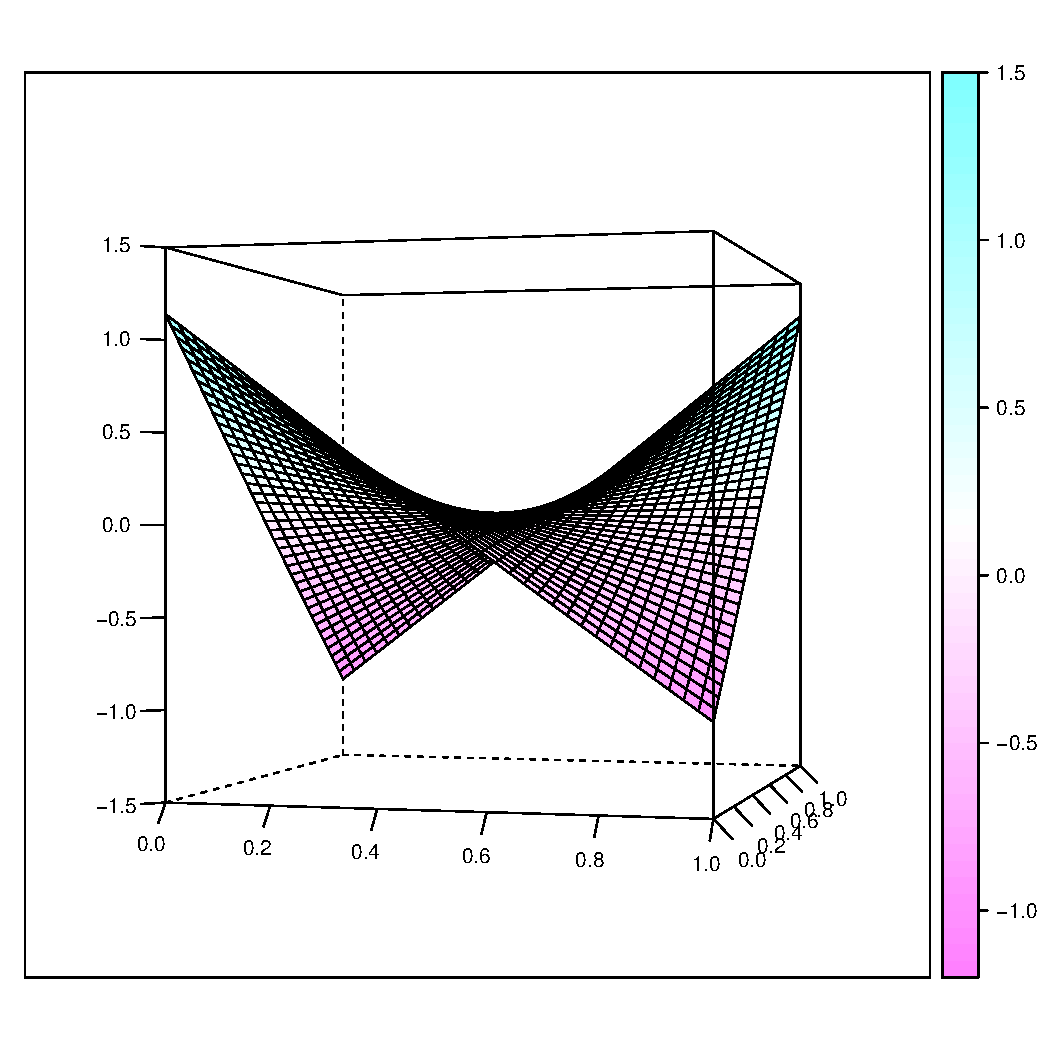
\includegraphics[width= 
		\textwidth]{Images-nonparametric/cy-fit-wireframe-m5.pdf} \caption{m = 5} \label{} 
	\end{subfigure}
	\begin{subfigure}
		[b]{0.40\textwidth} \centering 
		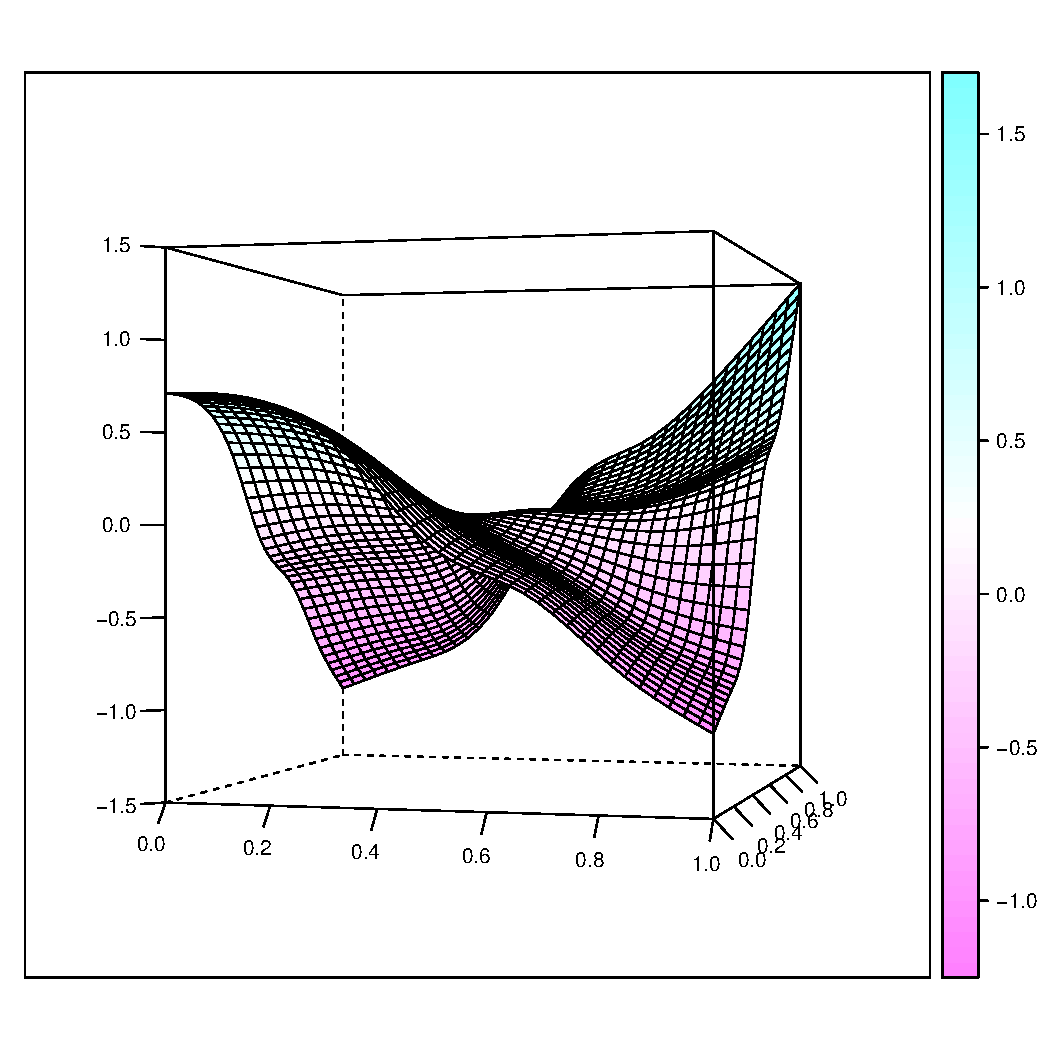
\includegraphics[width= 
		\textwidth]{Images-nonparametric/cy-fit-wireframe-m10.pdf} \caption{m = 10} \label{} 
	\end{subfigure}
	\begin{subfigure}
		[b]{0.40\textwidth} \centering 
		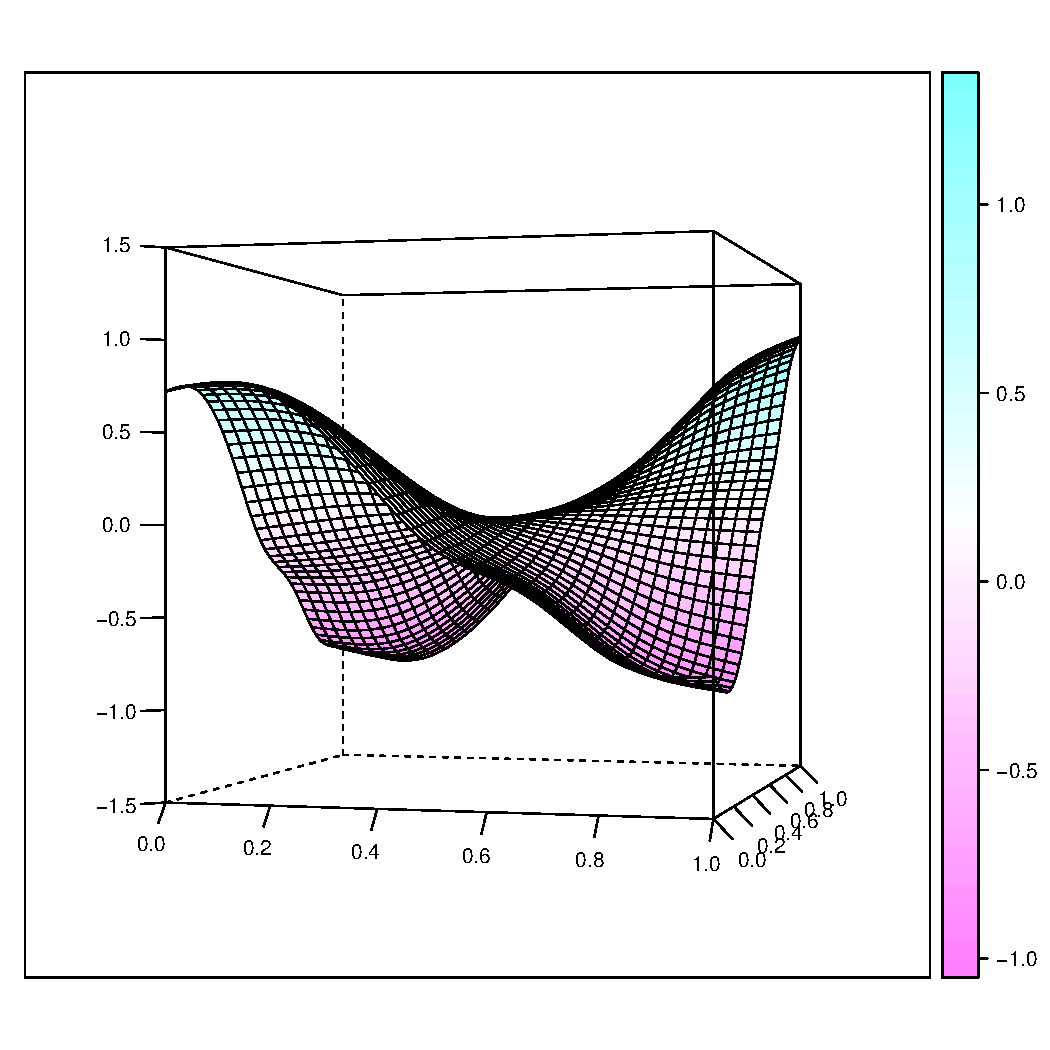
\includegraphics[width= 
		\textwidth]{Images-nonparametric/cy-fit-wireframe-m40.pdf} \caption{m = 20} \label{} 
	\end{subfigure}
	\begin{subfigure}
		[b]{0.40\textwidth} \centering 
		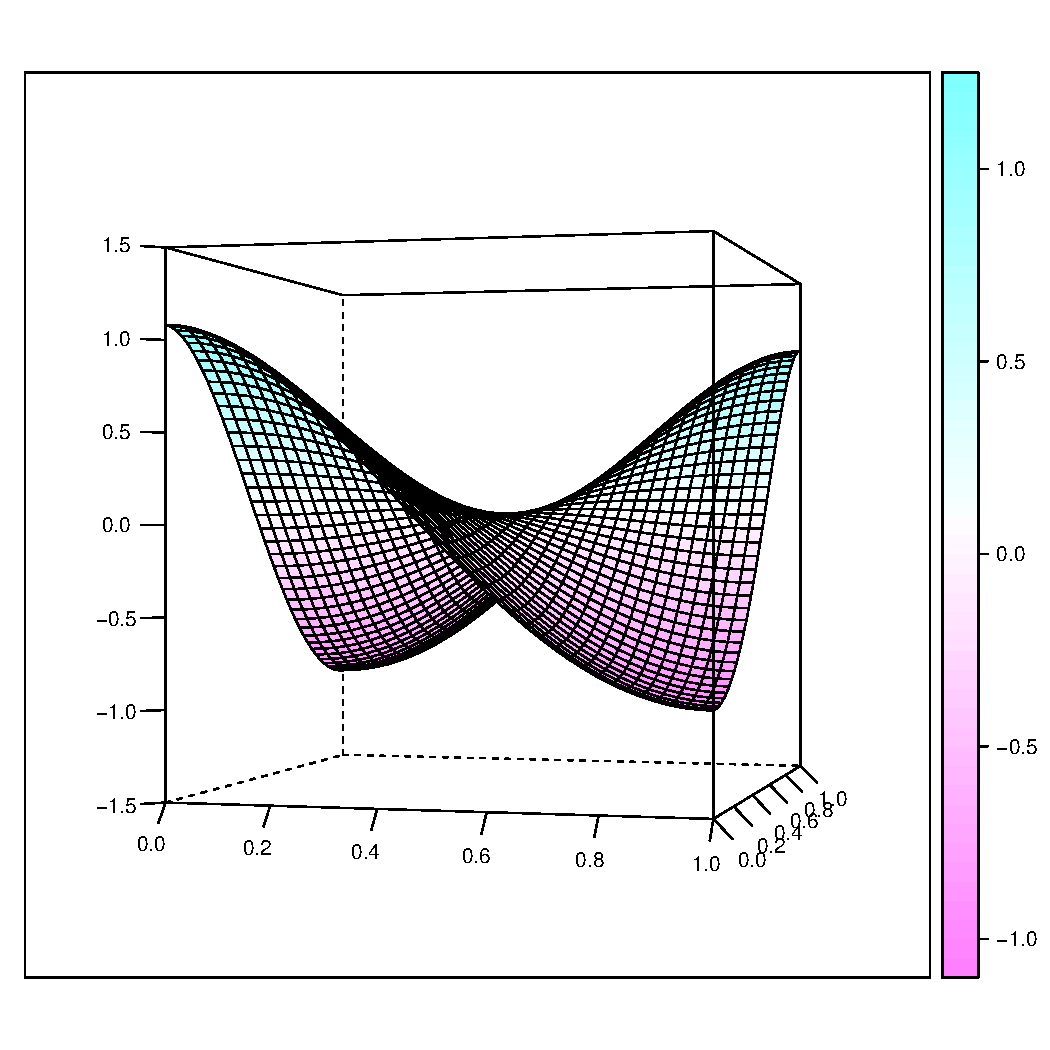
\includegraphics[width= 
		\textwidth]{Images-nonparametric/cy-true-wireframe.pdf} \caption{truth} \label{} 
	\end{subfigure}
	\caption{Estimated covariance functions using the SSCOV method an a data set consisting of 100 curves simulated from the process $X(t)$ in \eqref{eq:sim process} using observation standard deviation equal to $\sigma_0 = 0.329$. Here $m$ equals the number of observations for each curve. } \label{fig:covfits} 
\end{figure}

As an illustration, the fitted covariance function for a single simulated data set (under scenario I) is shown in Figure \ref{fig:covfits}. To understand the general performance of the FPC estimator, we repeated this process 100 times using 100 curves with $\sigma_0=0.369$, resulting in a signal to noise ratio of $2:1$. Figures \ref{fig:fpca-ss-1} and \ref{fig:fpca-fda-1} show the pointwise mean and pointwise central 95\% quantile of the first two estimated functional principal components under senario 1. Figures \ref{fig:fpca-ss-2} and \ref{fig:fpca-fda-2} show results from scenario II, Figures \ref{fig:fpca-ss-3} and \ref{fig:fpca-fda-3} show results from scenario III. Estimation error measured by integrated square error is summarized in Table \ref{tab:fpc-norm}. 

The general wisdom is to avoid smoothing individual curves with sparse data; however, our simulations show that this approach performs adequately when the `time' observations are uniformly distributed (i.e. scenario I) with respect to integrated squared error (see Table \ref{tab:fpc-norm}). Visual inspection of the error bands in Figure \ref{fig:fpca-fda-1} and Figure \ref{fig:fpca-fda-2} indicate that the SIC method tends to produce an overly smooth estimate, particularly for the sparse case where the second functional principal component is well outside the error bands. Visual inspection also indicates increased variation in the SSCOV method compared to the SIC method, though the variation is consistent with the true curve. It is also clear that the effect of sampling frequency $m$ on the magnitude of the variation is less pronounced in the SSCOV method. This makes sense due to the fact that the SSCOV method pools data before estimation, thus even the sparse case ($m = 5$) results in a large number of observations when pooled across 100 curves. 

The most striking difference in performance between the two methods was when we allowed the `time' points for each curved to be generated from different beta distributions (scenario III). The skewed and U-shaped distributions can severely restrict across-the-curve information, and it is clear from Figure \ref{fig:fpca-fda-3} that the SIC method performs poorly at estimating the second functional principal component. By pooling all the data the SSCOV method still performs adequately in this scenario. 
\begin{table}
	[ht] \caption{Average integrated squared error $\norm{\hat{\psi}(t) - \psi(t)}^2_{L_2}$: averaged over 100 runs. The Monte Carlo standard error is shown in parentheses.} \centering 
	\begin{tabular}
		{|c|c|l|cc|} \hline Scenerio & FPC & m & SSCOV & SIC \\
		\hline \multirow{6}{*}{I}& \multirow{3}{*}{1st} & 5 & 0.0231 (0.0018) & 0.0150 (0.0011) \\
		& & 10 & 0.0142 (0.0009) & 0.0059 (0.0003) \\
		& & 20 & 0.0064 (0.0005) & 0.0024 (0.0002) \\
		\cline{2-5} & \multirow{3}{*}{2nd} & 5 & 0.9750 (0.0727) & 0.8112 (0.0316) \\
		& & 10 & 0.4861 (0.0529) & 0.1401 (0.0110) \\
		& & 20 & 0.1148 (0.0113) & 0.0408 (0.0028) \\
		\hline \multirow{6}{*}{II}& \multirow{3}{*}{1st} & 5 & 0.0241 (0.0015) & 0.0228 (0.0026) \\
		& & 10 & 0.0154 (0.0013) & 0.0068 (0.0006) \\
		& & 20 & 0.0084 (0.0007) & 0.0026 (0.0002) \\
		\cline{2-5} & \multirow{3}{*}{2nd} & 5 & 0.9866 (0.0723) & 1.0775 (0.0344) \\
		& & 10 & 0.4918 (0.0493) & 0.3004 (0.0268) \\
		& & 20 & 0.2484 (0.0342) & 0.0545 (0.0054) \\
		\hline \multirow{6}{*}{III} & \multirow{3}{*}{1st} & 5 & 0.0215 (0.0014) & 0.2713 (0.0298) \\
		& & 10 & 0.0166 (0.0015) & 0.0436 (0.0044) \\
		& & 20 & 0.0116 (0.0012) & 0.0173 (0.0018) \\
		\cline{2-5} & \multirow{3}{*}{2nd} & 5 & 1.2658 (0.0608) & 1.8348 (0.0077) \\
		& & 10 & 0.9027 (0.0570) & 1.6777 (0.0080) \\
		& & 20 & 0.6024 (0.0519) & 1.4112 (0.0119) \\
		\hline 
	\end{tabular}
	\label{tab:fpc-norm} 
\end{table}
\begin{figure}
	\begin{center}
		\begin{tabular}
			{ccc} $m$ = 5 & $m$ = 10 & $m$ = 20 \\
			\includegraphics[width=2in]{Images-nonparametric/sim-study/fpc1-fpca-ss-params-ind-5.pdf} & 
			\includegraphics[width=2in]{Images-nonparametric/sim-study/fpc1-fpca-ss-params-ind-10.pdf} & 
			\includegraphics[width=2in]{Images-nonparametric/sim-study/fpc1-fpca-ss-params-ind-20.pdf} \\
			\includegraphics[width=2in]{Images-nonparametric/sim-study/fpc2-fpca-ss-params-ind-5.pdf} & 
			\includegraphics[width=2in]{Images-nonparametric/sim-study/fpc2-fpca-ss-params-ind-10.pdf} & 
			\includegraphics[width=2in]{Images-nonparametric/sim-study/fpc2-fpca-ss-params-ind-20.pdf} \\
		\end{tabular}
	\end{center}
	\caption{Functional principal component estimation using the SSCOV method. For each of the 100 simulated data sets 100 curves were simulated with $m$ observations per curve using scenario I. The solid line is the pointwise mean, the dashed line is the true FPC, and the gray bands show the pointwise 2.5 and 97.5 quantiles.} \label{fig:fpca-ss-1} 
\end{figure}
\begin{figure}
	\begin{center}
		\begin{tabular}
			{ccc} $m$ = 5 & $m$ = 10 & $m$ = 20 \\
			\includegraphics[width=2in]{Images-nonparametric/sim-study/fpc1-fpca-fda-params-ind-5.pdf} & 
			\includegraphics[width=2in]{Images-nonparametric/sim-study/fpc1-fpca-fda-params-ind-10.pdf} & 
			\includegraphics[width=2in]{Images-nonparametric/sim-study/fpc1-fpca-fda-params-ind-20.pdf} \\
			\includegraphics[width=2in]{Images-nonparametric/sim-study/fpc2-fpca-fda-params-ind-5.pdf} & 
			\includegraphics[width=2in]{Images-nonparametric/sim-study/fpc2-fpca-fda-params-ind-10.pdf} & 
			\includegraphics[width=2in]{Images-nonparametric/sim-study/fpc2-fpca-fda-params-ind-20.pdf} \\
		\end{tabular}
	\end{center}
	\caption{Functional principal component estimation using the SIC method as described in \cite{FDA}. For each of the 100 simulated data sets 100 curves were simulated with $m$ observations per curve using scenario I. The solid line is the pointwise mean, the dashed line is the true FPC, and the gray bands show the pointwise 2.5 and 97.5 quantiles.} \label{fig:fpca-fda-1} 
\end{figure}

%%%%%%%%%%%%%% Missing Gap data %%%%%%
\begin{figure}
	\begin{center}
		\begin{tabular}
			{ccc} $m$ = 5 & $m$ = 10 & $m$ = 20 \\
			\includegraphics[width=2in]{Images-nonparametric/sim-study/fpc1-gap-fpca-ss-params-ind-5.pdf} & 
			\includegraphics[width=2in]{Images-nonparametric/sim-study/fpc1-gap-fpca-ss-params-ind-10.pdf} & 
			\includegraphics[width=2in]{Images-nonparametric/sim-study/fpc1-gap-fpca-ss-params-ind-20.pdf} \\
			\includegraphics[width=2in]{Images-nonparametric/sim-study/fpc2-gap-fpca-ss-params-ind-5.pdf} & 
			\includegraphics[width=2in]{Images-nonparametric/sim-study/fpc2-gap-fpca-ss-params-ind-10.pdf} & 
			\includegraphics[width=2in]{Images-nonparametric/sim-study/fpc2-gap-fpca-ss-params-ind-20.pdf} \\
		\end{tabular}
	\end{center}
	\caption{Functional principal component estimation using the SSCOV method. For each of the 100 simulated data sets 100 curves were simulated with $m$ observations per curve using scenario II. The solid line is the pointwise mean, the dashed line is the true FPC, and the gray bands show the pointwise 2.5 and 97.5 quantiles.} \label{fig:fpca-ss-2} 
\end{figure}
\begin{figure}
	\begin{center}
		\begin{tabular}
			{ccc} $m$ = 5 & $m$ = 10 & $m$ = 20 \\
			\includegraphics[width=2in]{Images-nonparametric/sim-study/fpc1-gap-fpca-fda-params-ind-5.pdf} & 
			\includegraphics[width=2in]{Images-nonparametric/sim-study/fpc1-gap-fpca-fda-params-ind-10.pdf} & 
			\includegraphics[width=2in]{Images-nonparametric/sim-study/fpc1-gap-fpca-fda-params-ind-20.pdf} \\
			\includegraphics[width=2in]{Images-nonparametric/sim-study/fpc2-gap-fpca-fda-params-ind-5.pdf} & 
			\includegraphics[width=2in]{Images-nonparametric/sim-study/fpc2-gap-fpca-fda-params-ind-10.pdf} & 
			\includegraphics[width=2in]{Images-nonparametric/sim-study/fpc2-gap-fpca-fda-params-ind-20.pdf} \\
		\end{tabular}
	\end{center}
	\caption{Functional principal component estimation using the SIC method as described in \cite{FDA}. For each of the 100 simulated data sets 100 curves were simulated with $m$ observations per curve using scenario II. The solid line is the pointwise mean, the dashed line is the true FPC, and the gray bands show the pointwise 2.5 and 97.5 quantiles.} \label{fig:fpca-fda-2} 
\end{figure}

%%%%%%%%%%%%%% BETA %%%%%%
\begin{figure}
	\begin{center}
		\begin{tabular}
			{ccc} $m$ = 5 & $m$ = 10 & $m$ = 20 \\
			\includegraphics[width=2in]{Images-nonparametric/sim-study/fpc1-beta-fpca-ss-params-ind-5.pdf} & 
			\includegraphics[width=2in]{Images-nonparametric/sim-study/fpc1-beta-fpca-ss-params-ind-10.pdf} & 
			\includegraphics[width=2in]{Images-nonparametric/sim-study/fpc1-beta-fpca-ss-params-ind-20.pdf} \\
			\includegraphics[width=2in]{Images-nonparametric/sim-study/fpc2-beta-fpca-ss-params-ind-5.pdf} & 
			\includegraphics[width=2in]{Images-nonparametric/sim-study/fpc2-beta-fpca-ss-params-ind-10.pdf} & 
			\includegraphics[width=2in]{Images-nonparametric/sim-study/fpc2-beta-fpca-ss-params-ind-20.pdf} \\
		\end{tabular}
	\end{center}
	\caption{Functional principal component estimation using the SSCOV method. For each of the 100 simulated data sets 100 curves were simulated with $m$ observations per curve using scenario III. The solid line is the pointwise mean, the dashed line is the true FPC, and the gray bands show the pointwise 2.5 and 97.5 quantiles.} \label{fig:fpca-ss-3} 
\end{figure}
\begin{figure}
	\begin{center}
		\begin{tabular}
			{ccc} $m$ = 5 & $m$ = 10 & $m$ = 20 \\
			\includegraphics[width=2in]{Images-nonparametric/sim-study/fpc1-beta-fpca-fda-params-ind-5.pdf} & 
			\includegraphics[width=2in]{Images-nonparametric/sim-study/fpc1-beta-fpca-fda-params-ind-10.pdf} & 
			\includegraphics[width=2in]{Images-nonparametric/sim-study/fpc1-beta-fpca-fda-params-ind-20.pdf} \\
			\includegraphics[width=2in]{Images-nonparametric/sim-study/fpc2-beta-fpca-fda-params-ind-5.pdf} & 
			\includegraphics[width=2in]{Images-nonparametric/sim-study/fpc2-beta-fpca-fda-params-ind-10.pdf} & 
			\includegraphics[width=2in]{Images-nonparametric/sim-study/fpc2-beta-fpca-fda-params-ind-20.pdf} \\
		\end{tabular}
	\end{center}
	\caption{Functional principal component estimation using the SIC method as described in \cite{FDA}. For each of the 100 simulated data sets 100 curves were simulated with $m$ observations per curve using scenario III. The solid line is the pointwise mean, the dashed line is the true FPC, and the gray bands show the pointwise 2.5 and 97.5 quantiles.} \label{fig:fpca-fda-3} 
\end{figure}

% section simulations (end)
\section{Conclusions} 

% (fold)
\label{sec:conclusions}

We have shown how the reproducing kernel Hilbert space framework for covariance estimation can be extended to allow the use of function spaces where the penalty functional induces a non-empty unpenalized subspace. We have also derived a functional principal component estimator for this case. Even though development here was for a specific penalty, the method is very general and could easily be applied to other penalties, though the form of the reproducing kernel and the basis for the null space will depend on this choice. 

Our simulations show that this method performs well even when sampling points on each curve do not follow a common distribution on $\T$. The robustness to the assumption of common distribution is encouraging as longitudinal data often do not satisfy this assumption. It is somewhat surprising that this method does not seem to perform much better than standard methods in terms of integrated squared error in the other scenerios as can be seen in Table \ref{tab:fpc-norm}. However, there appears to be a clear difference in terms of bias in estimating the second FPC, particularly in the sparse case (m = 5). The standard method over smoothes in this case as the true seoncd FPC is far outside the error bands.   

We have also created an R package implementation of this method with user-friendly functions for estimating the covariance function and principal component functions for functional data, making it convenient to use empirical basis representation for functional data analyses. 

% section conclusions (end)
\section{Proofs} 

% (fold)
\label{sec:proofs}

Proof of Lemma \ref{thm:eigenfunctions} 
\begin{proof}
	Let $\theta_k$ be the eigenvalues of $Q^{1/2}AQ^{1/2}$, then 
	\begin{align*}
		\sum \theta_k \hat{\psi}_k(s)\hat{\psi}_k(t) &= \sum \theta_kb'_k\mathbf{g}(s)b'_k\mathbf{g}(t) \\
		&= \sum \theta_k\mathbf{g}'(s)b_kb'_k\mathbf{g}(t) \\
		&= \mathbf{g}'(s)\left( B 
		\begin{bmatrix}
			\theta_1 & & &\\
			& \ddots &\\
			& & \theta_k 
		\end{bmatrix}
		B' \right) \mathbf{g}(t). 
	\end{align*}
	To complete the proof, we show that $B 
	\begin{bmatrix}
		\theta_1 & & &\\
		& \ddots &\\
		& & \theta_k 
	\end{bmatrix}
	B'=A$, 
	\begin{align*}
		B 
		\begin{bmatrix}
			\theta_1 & & &\\
			& \ddots &\\
			& & \theta_k 
		\end{bmatrix}
		B' &= Q^{-1/2}U 
		\begin{bmatrix}
			\theta_1 & & &\\
			& \ddots &\\
			& & \theta_k 
		\end{bmatrix}
		U'Q^{-1/2}\\
		&= Q^{-1/2}[\theta_1\mathbf{u}_1| \dots |\theta_k\mathbf{u}_k] U'Q^{-1/2}\\
		&= Q^{-1/2}[Q^{1/2}AQ^{1/2}\mathbf{u}_1| \dots| Q^{1/2}AQ^{1/2}\mathbf{u}_k] U'Q^{-1/2}\\
		&= Q^{-1/2}Q^{1/2}AQ^{1/2}U U'Q^{-1/2}\\
		&= A. 
	\end{align*}
	Thus, $\sum \theta_k \hat{\psi}_k(s)\hat{\psi}_k(t) = g'(s)Ag(t) = \hat{C}(s,t)$. \qedhere 
\end{proof}

% section proofs (end) 



%!TEX root = ../dissertation.tex
\chapter{ESTIMATION AND KRIGING FOR SPATIALLY INDEXED FUNCTIONAL DATA} 
\label{ch:functional kriging}

\section{Introduction} 

% (fold)
\label{sec:introduction}
Data that arise from measurements at geographic locations often exhibit similarities at small spatial scales. When the primary objective of analysis is to predict values at unobserved locations, geostatistical models are particularly useful. When data are measurements from a ground-based sensor, there is often temporal component to the data, examples include: \cite{Kaiser:2002wna} who investigate the concentration of an air pollutant; Delaigle and Hall (2010) who consider Australian rainfall data; and the Canadian weather data showcased in Ramsay and Silverman (2005). When the temporal measurements are not regular in time its useful to treat the time process as functional data. The extension of geostatistical models for functional data were first considered in \cite{Goulard:1993} where two approaches are proposed: one approach involves cokriging by reducing the functional response to a multivariate response by modeling the spatial component through the coefficients of a parametric model, while the other approach utilizes a functional version of the variogram. The functional variogram approach has been further developed by \cite{Giraldo:2010jx}. We pursue the first option, but do not make the assumption of a parametric model for the curves. We allow the curves to be represented nonparametrically using a principal component function basis. Typically, very few principal component functions are needed to represent the major modes of variation in the curves, thus making a multivariate geostatistical approach feasible without the need of a parametric model. 



% \begin{figure}
% 	\begin{center}
% 		\includegraphics[width=0.7\textwidth]{images-ordinary-kriging/plot_from_Nerini2010.png}
% 	\end{center}
% 	\caption{Data set from \cite{Nerini:2010ba} modeling ocean temperatures collected by equipment attached to diving elephant seals.} \label{fig:nerini}
% \end{figure}

% section introduction (end)

% \section{Statistical model for spatially indexed functional data}
%
% % (fold)
% \label{sec:statistical_model_for_spatially_indexed_functional_data}
%
% We work with data consisting of curves $X(s_k; t),$ $t \in [0,T]$, at spatial locations $s_1, \dots, s_n$. We define a \emph{spatial functional process} as
% \[ \left\{ \boldsymbol X(s; t): s \in D \subseteq \Real^2, t \in \T \right\}, \]
% where, for fixed location $s_k$, $\boldsymbol X(s_k; \cdot)$ is a random function on the closed interval $\mathcal{T}$ taking values in a reproducing kernel Hilbert space of functions $\H$ with reproducing kernel $K(s,t)$ which is assumed to be square integrable. The requirement that the curves belong to a reproducing kernel Hilbert space instead of typical $L^p$ space has to do with the method we employ to estimate the principal component functions in section \ref{sec:eigenfunction_estimation}.
%
% The functions $X(s;t)$ admit the following representation
% \begin{equation}
% 	X(s;t) = \mu(t) + \epsilon(s;t),
% \end{equation}
% where $\mu(t)$ represents large-scale structure which does not depend on spatial location and $\epsilon(s;t)$ is a mean zero spatially correlated random effect. The methodology we propose assumes $\epsilon(s;t)$ can be represented by the Karhunen-Loeve expansion $\epsilon(s;t) = \sum_{k=1}^{\infty} \alpha_k(s)\psi_k(t)$. The functions $\psi_k(\cdot)$ are eigenfunctions of the covariance operator and are called the principal component functions (FPC). For each integer $k$, $\alpha_k(s) = \inner{\epsilon(s;t)}{ \psi_k(t)}$ is a scalar random field assumed to be a second-order stationary and isotropic. Spatial random fields connected to different FPCs are assumed to be uncorrelated, that is
% \begin{equation}
% 	\text{Cov}(\alpha_j(s), \alpha_l(s')) = 0 \hspace{1cm} \text{for } j \neq l. \label{eq:nocrosscor}
% \end{equation}
%
% For simplicity assume the functions are centered (i.e. $\mu(t)=0$), then under assumption \eqref{eq:nocrosscor}, the covariance between trajectories at locations $s_j$ and $s_l$ are given by
% \begin{align}
% 	\text{Cov}(X(s_j,t), X(s_l, t')) &= \sum_{k=1}^{\infty}\text{Cov}(\alpha_k(s_j), \alpha_k(s_l))\psi_k(t)\psi_k(t')\\
% 	&= \sum_{k=1}^{\infty}h_k(\norm{s_j-s_l})\psi_k(t)\psi_k(t'). \label{eq:cov}
% \end{align}
% Gromenko and Kokozka (2012) point out that assumption \eqref{eq:nocrosscor} is implied by a separable spatio-temporal covariance function, and is necessary to ensure positive definiteness. Further, it is clear from the form of the covariance function \eqref{eq:cov} that the spatial component is stationary, while the temporal component is nonstationary. From a practical viewpoint, assumption \ref{eq:nocrosscor} results in a fairly parsimonious model as it does not require modeling the cross covariances between coefficient random fields.
%
% In practice we work with the truncated expansion $\epsilon(s;t) = \sum_{k=1}^{q} \alpha_k(s)\psi_k(t)$, where $q$ is chosen to preserve most of the variation. Conventional wisdom stipulates that this means at least 85\% of the total variation is accounted for by the truncated expansion. Our experience suggests that often no more then 2-4 FPCs are need to capture 85\% of the variation, so this approach often reduces to a very low dimensional multivariate problem.
%
% % section statistical_model_for_spatially_indexed_functional_data (end)


\section{Ordinary kriging of function-valued data} % (fold)
\label{sec:ordinary_kriging_of_function_valued_data}
The ordinary kriging methodology described in this section was developed in \cite{Giraldo:2010jx}, and is a direct translation of the ordinary kriging from the scalar-valued data to function-valued data. Let $X_{s_1}(t), \dots, X_{s_n}(t)$ be realizations of the functional random process $X_s(t)$ at site $s_1, \dots, s_n$. For an unobserved location $s_0$, the predictor for $X_{s_0}$ is given by 
\begin{equation}
	\hat{X}_{s_0} = \sum_{i=1}^n\lambda_i X_{s_i}(t) \mbox{\hspace{0.5cm}} \lambda_i, \dots, \lambda_n \in \mathbb{R} \label{OKFD predictor}
\end{equation}
The following formal assumptions establish the stationarity conditions:
\begin{itemize}
	\item $E(X_s(t)) = \mu(t)$ and $Var(X_s(t)) = \sigma^2(t)$ for all $s \in D$ and $t \in [a,b]$
	\item $Cov(X_{s_i}(t), X_{s_j}(t)) = C(\norm{s_i - s_j})(t) = C_{ij}(h,t)$, where $h = \norm{s_i - s_j}$.
	\item $\frac{1}{2}Var(X_{s_i} - X_{s_j}) = \gamma(\norm{s_i - s_j})(t) = \gamma(h,t)$
\end{itemize}
The estimator in \eqref{OKFD predictor} is a linear predictor and the weights $\lambda_i$ are derived such that the predictor is the best linear unbiased predictor (BLUP). The unbiased constraint requires that $\sum_{i=1}^n\lambda_i = 1$, and the BLUP is obtained by minimizing
\begin{equation}
	\sigma^2_{s_0} = Var(\hat{X}_{s_0} - X_{s_0}).
\end{equation}
Implementation of this method requires a preprocessing step involving non-parametric fitting of the observed data to achieve smooth representations of the functions $X_{s_1}(t), \dots, X_{s_n}(t)$. This is accomplished by fitting a finite b-spline basis where the dimension of the basis and the smoothing parameter are chosen by a functional cross-validation algorithm. 
% section ordinary_kriging_of_function_valued_data (end)

\section{Cokriging functional principal components scores} % (fold)
\label{sec:cokriging_functional_principal_compents_scores}
In the method described in the previous section, the set of curves are modeled directly as a spatial random field. The approach we describe here is fundamentally different in that the spatial model is defined on the coefficient vectors corresponding to a finite basis expansion. The coefficient vector is often low dimensional, as each curve is represented as a linear combination of the leading functional principal components. To guarantee such a representation exists and can be estimated efficiently requires assumptions on the function space itself, which we describe here. 
  We model trajectories $X_s(t)$ as a continuos second order stochastic process with mean $\mu(t)$ and bivariate temporal covariance function
\begin{equation}
	C_{0}(t',t)=E([X(t')-\mu(t')][X(t)-\mu(t)]),\mbox{ }\forall t',t\in \T=[a,b]. 
\end{equation} 
 We assume the underling trajectories $X_s(t)$ are smooth in that they take values in the reproducing kernel Hilbert space $\H= \{f : f, f' \mbox{ absolutely continuous}, f'' \in L_2[\T]\}$, with inner product $\inner{f}{g}_{\H}$ described in \eqref{inner prod}.

Let $X_{s_1}(t), \dots, X_{s_n}(t)$ represent the collection of realizations of $X_s(t)$. The data we consider are finite observations of each curve corrupted by noise. The model for the observed values $Y_s(t_{ij})$ is described by,
\begin{equation}
	Y_s(t_{ij})=X_s(t_{ij})+\epsilon_{ij},\mbox{ }j=1,\dots,m;\mbox{ }i=1,\dots,N, \label{kriging:observation model}
\end{equation} 
where $i$ indexes spatial location and $j$ indexes the finite observations on a single trajectory. The `time' observations are not assumed to be the same across curves; that is, $t_{ij}$ does not necessarily equal $t_{i'j}$ for $i \neq i'$. To simplify notation we assume the number of observations on each curve, $m$, is consistent across curves though this assumption can be relaxed. The $\epsilon_{ij}$ are independently and identically distributed measurement errors with mean zero and finite variance $\sigma_{0}^{2}.$ It is further assumed that the random functions $X_s(t)$, and measurement errors $\epsilon$ are mutually independent. 

To simplify notation, assume $\mu(t)=0$, so that functions $X_s(t)$ admit the following representation 
\begin{equation}
	X_{s}(t) = \sum_{k=1}^{q} \alpha_k(s)\psi_k(t) = \boldsymbol{\alpha}\boldsymbol{\psi}, \label{kriging: fpc expansion}
\end{equation}
where the functions $\psi_k(t)$ are eigenfunctions of the covariance function $C_0(t',t)$, and $\alpha_k(s) = \inner{X_s(t)}{ \psi_k(t)}_{\H}$. The value of $q$ is determined such that at least 90\% of the variation in the curves is explained by the first $q$ FPCs. In this framework, predicting a curve at an unobserved location $s_0$ is achieved by predicting the corresponding coefficient vector $\boldsymbol{\alpha(s_0)}=[\alpha_1(s_0), \dots, \alpha_q(s_0)]$. This approach requires two separate tasks: estimating the functional principal components, and modeling the coefficient random fields. Section \ref{sub:FPC estimation} describes our method for estimating FPCs, and Section \ref{sec:functional_kriging_predictor} describes our approach to prediction by modeling the coefficients as a multivariate spatial random field.
% subsection subsection_name (end)
\subsection{Estimation} % (fold)
\label{sub:estimation}

% subsection estimation (end)
We achieve smooth versions of the underlying trajectories $X_s(t)$ by expressing them as a finite basis expansion of principal component functions corresponding the the covariance function $C_0(t',t)$. The covariance of the observational process $Y_{ij}$ is given by
\begin{equation}
	C(Y_i(t_{ij}), Y_i(t_{ik})) = C_0(X_i(t_{ij}), X_i(t_{ik})) + \sigma^2_0 \delta_{jk}
\end{equation}
where $\delta_{jk}$ equals 1 if $j=k$ and is equal to zero otherwise. The covariance function $C_0(t',t)$ is recovered by performing bivariate smoothing on the sample covariance omitting the diagonal values.  The covariance function estimator we use is described in Chapter \ref{ch:covariance estimation} and is a modified version of the one proposed in \cite{Cai:2010vr} who show that this method has many desirable theoretical properties. The methodology, which is described in detail in described in Chapter \ref{ch:covariance estimation}, achieves both efficient estimation of $C_0(t',t)$ and results in closed-form estimates of corresponding FPCs.

\subsubsection{Covariance Estimation for independent curves} % (fold)
\label{sub:subsection_name}

% subsection subsection_name (end)
In this section we describe a nonparametric estimator for the covariance function $C_0(t',t)$ based on a collection $X_{s_1}(t), \dots, X_{s_n}(t)$ of independent realizations of the functional process $X_s(t)$. Let $\mathbf{b}^{(i)} = [(Y_i(t_{ij})-\mu(t_{ij}))(Y_i(t_{ij'})-\mu(t_{ij'}))]_{1\leq j\neq j'\leq m}$, $i=1, \dots, N$; $j,j' \in 1, \dots, m$. Further, let
\begin{equation}
	\mathbf{b} = (\mathbf{b}^{(1)T}, \mathbf{b}^{(2)T}, \dots, \mathbf{b}^{(n)T} )^T, \label{b}
\end{equation} 
where the column vectors $\mathbf{b}^{(i)}$ contain all pairwise products of observations on the $i$th curve, excluding those that are the product of an observation with itself which correspond to the diagonal values on $[0,1]\times [0,1]$. The column vector $\mathbf{b}$ contains all the information in the sample about the covariance function. Using this notation the covariance estimator is defined by the following optimization problem,
\begin{equation}
	 \widehat{C}_{\lambda}=\stackrel[C \in \H\otimes \H]{}{\text{ argmin}} \left\{\frac{1}{nm^2-nm} (\mathbf{b} - \mathbf{C})^T(\mathbf{b} - \mathbf{C})+\lambda\left\Vert C\right\Vert _{\breve{\H}}^{2} \right\},
	 \label{kriging: cov est}
	 \end{equation}
where
\[ \mathbf{C} = [C(t_{ij}, t_{ij'})], \]
 $\lambda$ is a smoothing parameter estimated using cross validation, and $\breve{\H}$ is a subspace of $\H\tprod\H$. Details about the Hilbert space structure of $\H\tprod\H$ and form of the estimator see Chapter \ref{ch:covariance estimation}. 

\subsubsection{Covariance Estimation for spatially dependent curves} % (fold)
\label{sub:weighted covariance}

The covariance function estimator \eqref{kriging: cov est} assumes independent observations. Using this estimator with spatially correlated data may have an affect on bias, variance, or result in an estimator that is not consistent. In this section we introduce a computationally efficient way to adjust for some of the effects of spatial dependence on the covariance estimator \ref{kriging: cov est} using a weighting scheme motivated by the fundamental principle in spatial statistics: data in closer proximity have stronger correlation and contribute similar information. For irregularly spaced data, this can cause a bias toward the behavior of observations that are clustered together and are over represented in the sample. Here we describe an approach to counteract this tendency by down weighting curves where location intensity (i.e., number of locations per unit area) is high. Previous work on smoothing penalty based estimator like the one in \eqref{kriging: cov est} has shown that when the dependence assumption is violated, the estimator tends to under-smooth (\cite{Wang:1998tq}). The approach we consider here does not address the selection of the smoothing parameter directly, but reduces the influence of the highly correlated observations on estimation. 

Our approach involves creating a scalar weight for each curve based on location intensity and the strength of the correlation. The goal is to down-weight observations from highly correlated data because they provide redundant information. This approach is computationally efficient because it does not require computing the inverse of a high dimensional matrix---which is not feasible with the dimension of $\mathbf{b}$ in \eqref{b}.  

In order to quantify the conceptual approach described in the previous paragraph we proceed by estimating the point intensity at each location. Denote the estimated point intensity at location $k$ by $\gamma_k$ and define a weight function 
\begin{equation}
	w_k = \left(\frac{1}{\gamma_k}\right)^p, 
\end{equation}
where $p$ is a scale parameter connected to the strength of dependence.
Let $\mathbf{W}=diag(\mathbf{w}_1, \dots, \mathbf{w}_n)$, where $\mathbf{w}_i$ is a row vector whose length is equal to the length of $\mathbf{b}^{(i)}$ and whose components are all equal to $w_i$. The covariance estimator is adjusted by defining the loss function in \eqref{kriging: cov est} as 
\begin{equation}
	l_{n}(C)= (\mathbf{b} - \mathbf{C})^T\mathbf{W}(\mathbf{b} - \mathbf{C}). \label{eq:diag weighted loss function} 
\end{equation}
Note that for independent data, the value $p = 0$ will give equal weights and result in an identity matrix, i.e.,$\mathbf{W} = \mathbf{I}$. In Section \ref{sub:simulation covariance} we conduct a simulation study aimed at identifying optimal choice of $p$ under various spatial dependence scenarios. 

% To produce smooth estimates of the trajectories $X_i(t)$, project the observations $Y_i(t_j), j = 1, \dots, m$ onto the finite dimensional functional basis $\{\hat{\psi}_k(t), k = 1, \dots, q\}$, where $q$ is chosen such that at least $90\%$ of the variation is accounted for. The fitted trajectories admit the following representation
% \begin{equation}
% 	\widehat{X_i(t)} = \sum_{k=1}^q\alpha_{k,i} \hat{\psi}_k(t) = \boldsymbol{\alpha_i'}\boldsymbol{\psi}.
% 	\label{phen:coef}
% \end{equation}
% In this representation the randomness associated with each random trajectory $X(t)$ is captured in the coefficient vector $\boldsymbol{\alpha}$. In Section \ref{sub:land_cover_classification} the coefficients are treated as features in a classification model for land cover type. 

% section cokriging_functional_principal_compents_scores (end)
% section functional_kriging_methods (end)


% (fold)
\subsubsection{Functional Principal Component Estimation} % (fold)
\label{sub:FPC estimation}

% subsection subsection_name (end)
One of the practical benefits of the covariance estimator in \eqref{kriging: cov est} is that closed form expressions for the principal component functions can be computed. The methodology we describe here was developed in Chapter \ref{ch:covariance estimation}.

Functional principal components are related to the well-known Karhunen-Loeve representation theorem. For a square-integrable stochastic process $X(t)$ defined on a closed interval $[a,b]$, with continuous covariance $C(t',t)$, there is a corresponding linear operator $[T_Cf](t') = \int_a^bC(t',t)f(t)dt$. Since $C(t',t)$ is symmetric and non-negative definite, it has the following representation 

%(see Mercer's theorem)
\begin{equation*}
	C(t',t) = \sum_{i=1}^{\infty}\lambda_i\psi_i(t')\psi_i(t), 
\end{equation*}
where $\{\psi_m(t)\}_{m=1,2,\ldots}$ are a sequence of orthonormal eigenfunctions which form a complete basis in $L^2[a,b]$, and $\{\lambda_m \}_{m=1,2,\ldots}$ are nonnegative and nondecreasing eigenvalues. The eigenfunction-eigenvalue pair $\{\lambda_j, \psi_j(t)\}$ satisfy $\int_a^bC(t',t)\psi_j(t)dt = \lambda_j\psi_j(t)$, in other words the FPCs $\{\psi_j(t)\}$ are eigenfunctions of the covariance operator. The Karhunen-Loeve theorem states that the process $X(t)$ admits the representation 
\begin{equation*}
	X(t) = \sum_{m=1}^{\infty}\alpha_m \psi_m(t), \mbox{ where } \alpha_m = \int_a^b X(t) \psi_m(t)dt, 
\end{equation*}
and the random variables $\{\alpha_m \}_{m=1,2,\ldots}$ are uncorrelated and satisfy $E(\alpha_m)=0$ and Var($\alpha_m$) = $\lambda_m$, $\sum_m \lambda_m < \infty$. The eigenfunctions $\{\psi_m(t)\}_{m=1,2,\ldots}$ corresponding to $C(t',t)$ are the principal component functions and the coefficients $\{\alpha_m \}$ are the functional principal component scores of $X(t)$.

We seek functions $\hat{\psi}(s)$ that satisfy satisfy 
\begin{equation}
	\label{eq:eigenfuns} \int \hat{C}(t',t)\hat{\psi}(t)dt=\theta\hat{\psi}(t'). \nonumber
\end{equation}
The following Lemma which is Lemma \ref{thm:eigenfunctions} in Chapter \ref{ch:covariance estimation} states that the eigenfunction are linear combinations of function derived from the reproducing kernel on $\H$. 
\begin{lemma}
	\label{thm:eigenfunctions2} The eigenfunctions of $\hat{C}(t',t)$ can be expressed as 
	\begin{equation*}
		\hat{\psi}_k(\cdot) = \mathbf{b}'_k\mathbf{g}(\cdot), 
	\end{equation*}
	where $b_k$ is the $k$-th column of $B=Q^{-1/2}U$ and $U$ is the eigenvectors of $Q^{1/2}AQ^{1/2}$, and
	\[ \mathbf{g(\cdot)}=(1, k_1(\cdot),R_{1}(\cdot, t_1),R_{1}(\cdot, t_2),\dots, R_{1}(\cdot, t_K))'. \]
\end{lemma}
The exact form of the reproducing kernel on $\H$ is described in \ref{ch:covariance estimation}. In the Lemma \ref{thm:eigenfunctions2} the value $K$ is connected to the number of knot locations used for covariance estimation. See Section \ref{sub:practical_considerations_for_knot_selection} for recommendations on knot selection.

% section eigenfunction_estimation (end)
\subsection{Prediction} 

% (fold)
\label{sec:functional_kriging_predictor}

Using the functional principal components representation of $X_s(t)$ from \eqref{kriging: fpc expansion},
\begin{equation}
	X_{s}(t) = \sum_{k=1}^{q} \alpha_k(s)\psi_k(t) = \boldsymbol{\alpha}(s)\boldsymbol{\psi}, 
\end{equation}
the objective of constructing the best linear unbiased predictor of $X_{s_0}(t)$ and unobserved location $s_0$ is reframed as constructing the best linear unbiased predictor of the vector $\balpha_{s_0}$ given $\balpha(s_1), \dots, \balpha(s_n)$. We model $\balpha(s)$ as a stationary random field. A linaer predictor of the multivariate data $\balpha(s_1), \dots, \balpha_{s_1}$ has the form
\begin{equation}
	\hat{\balpha}(s_0) = \sum_{i=1}^n \balpha(s_i)\Gamma_i \label{kriging:predictor}
\end{equation}
where $\Gamma_i$ is a $q \times q$ matrix with $ij^{th}$ element equal to $\lambda_{ij}$. 
\begin{equation}
		\hat{\balpha}(s_0) = \sum_{i=1}^n [\alpha_1(s_i), \dots, \alpha_q(s_i)] 
		\left[ 
			\begin{array}{ccc}
				\lambda^i_{11} & \dots & \lambda^i_{1q}\\
				\vdots & \ddots & \vdots \\
				\lambda^i_{q1} & \dots & \lambda^i_{qq}
			\end{array}
		\right]
		\label{kriging:predictor 2}
\end{equation}
From \eqref{kriging:predictor 2} it is straight forward to derive the form of the components of $\hat{\balpha}(s_0)=[\hat{\alpha}_1(s_0), \dots, \hat{\alpha}_q(s_0)]$
\begin{equation}
	\hat{\alpha}_k(s_0) = \sum_{i=1}^n\sum_{j=1}^q\alpha_j(s_i)\lambda^i_{jk}, \mbox{ } k = 1, \dots, q.
\end{equation}
The off-diagonal values, $\lambda^i_{jk}$ $j \neq k$, are connected to the cross-covariance of the scalar random fields $\alpha(s)$ and are all equal to zero for a process with no cross-covariance; that is, under the assumption that $Cov(\alpha_j(s), \alpha_k(s)) = 0$ for $j \neq k$
\begin{equation}
	\lambda^i_{jk} = \begin{cases}
														0 & \text{ if } j \neq k\\
														\sum_{jj}^i = 1 & \text{for each $j$}\\
 										\end{cases}
\end{equation}

This shows that for an isotopic process with no cross-correlation, the kriging predictor is equivalent to kriging the components (\cite{wackernagel2003multivariate}, Ch. 25). Thus the problem of kriging a function is equival to univariate kriging of scalar coefficients. 

% Steps for prediction at unobserved location $s_0$:
% \begin{enumerate}
% 	\item Estimate the principal component functions, $\hat{\psi}^{(1)}, \hat{\psi}^{(2)}, \dots, \hat{\psi}^{(q)}$, choosing $q$ to account for at least 90\% of the total variation.
% 	\item Compute the projection of sample curves onto principal component functions
% 	\item Perform standard scalar-valued geostatistical analysis by fitting variograms to each scalar coefficient field.
% 	\item Compute kriged estimates of the coefficients: $\hat{\alpha}_{s_0}^{(1)}, \hat{\alpha}_{s_0}^{(2)}, \cdots, \hat{\alpha}_{s_0}^{(q)}$ .
% 	\item The functional cokriging predictor of the curve at location $s_0$ is given by
% 	\begin{equation}
% 		\widehat{X}_{s_0}(t)_{ok} = \sum_{k=1}^{q} \hat{\alpha}_{s_0}^{(k)}\hat{\psi}^{(k)}(t).
% 	\end{equation}
	
	%\todo{describe variance of the estimator}
%\end{enumerate}


% section functional_kriging_predictor (end)

\section{Simulation Studies} 

% (fold)
\label{sec:numerical_experiments}

In this section we conduct investigations using simulated data. We generate functional data as
\begin{equation}
	X_s(t) = \sum^{3}_{k=1}\zeta_k Z_k(s) \cos(k\pi t) \hspace{0.5cm} t \in [0,1], 
	\label{eq:sim process2} 
\end{equation}
where \(\zeta_k=(-1)^{k+1}k^{-2}\). The random variables $Z_k(s)$ are sampled from a Gaussian random field with $E[Z_k(s)]=0$ and 
\begin{equation}
	Cov(Z_k(s_i), Z_j(s_l)) = \begin{cases} 
																e^{-\norm{s_i - s_l}/r} &\mbox{ if } k = j\\
																0 & \mbox{ if } j \neq k.
															\end{cases}
	\label{eq:exp cov}
\end{equation} 
The range parameter, $r$, in the exponential covariance in equation \eqref{eq:exp cov} controls the strength of spatial dependence. 

\subsection{Simulation study of the spatially weighted covariance function estimator} % (fold)
\label{sub:simulation covariance}

In this simulation study we investigate the effect of adjusting the covariance function estimator for spatial dependence by simulating curves from the three different sets of locations shown in Figure~\ref{fig:grid3}. Different degrees of spatial dependence are controlled by the range parameter $r$ in \eqref{eq:exp cov} of the Gaussian random fields, $Z_i$, in \eqref{eq:sim process2}. Figure~\ref{fig:exp_corr_funs} shows the exponential correlation functions that correspond to the range values: $r = 0.0, 0.1, 0.2, 0.3, 0.4$, ranging from independence (r = 0) to strong spatial dependence (r = 0.4).

In order to gain insight into the performance of the covariance estimator in \eqref{eq:diag weighted loss function} simulate functional data sets using the observation model 
\begin{equation}
	Y^{(k)}_{ij}(t_{ij}) = X_{ij}(t_{ij}) + \epsilon_{ij}, \mbox{ } i = 1, \dots, 68;\; j = 1, \dots, 20;\; k = 1, \dots, 100,
\end{equation}
where $\epsilon_{ij} \sim N(0, 0.01^2)$ and the superscript $k$ indexes simulated data sets. The number of observations per curve and observation error variance are fixed. 

For each simulated data set, $Y^{(k)}$, the integrated squared difference between the estimated and true covariance function is calculated. We define the quantity $L$ to be the average integrated squared difference
\begin{equation}
	L = \frac{1}{100}\sum_{k=1}^{100}\int_{[0,1]^2} [\hat{C}^{(k)}(t_1, t_2) - C(t_1,t_2)]^2dt_1dt_2.
\end{equation}
The results of the simulations are shown in Figure~\ref{fig:MSE_trends}, where value of $L$ for each simulation scenario is plotted with lines connecting points with the same strength of spatial dependence. The spatial weights make more of an improvement on estimation for curves with stronger spatial correlation, though the optimal choice of the weight parameter appears to be near $1/2$ for all scenarios. We also note that very little estimation performance is sacrificed by using the spatial weights for independent curves for $p \leq 1/2$.

% plot of locations used to simulate curves
\begin{figure}[h]
	\begin{center}
		\includegraphics[width=\textwidth]{Images-ordinary-kriging/Plots/grids.pdf} 
	\end{center}
	\isucaption{Locations of curves used for the simulation.} \label{fig:grid3} 
\end{figure}

% plot of exponential covariance functions
\begin{figure}[h]
	\begin{center}
		\includegraphics[width=0.7\textwidth]{Images-ordinary-kriging/Plots/exp_corr_funs.pdf} 
	\end{center}
	\isucaption{Exponential covariance functions used in the simulation.} \label{fig:exp_corr_funs} 
\end{figure}

% plots of MSE vs spatial weight values for different values of spatial dependence
\begin{figure}[h]
	\begin{center}
		\includegraphics[width=\textwidth]{Images-ordinary-kriging/Plots/MSE_trends_all.pdf} 
	\end{center}
	\isucaption{The x-axis shows the value of the scale parameter, $p$, in the weight function. Large values of $p$ correspond to smaller weights for curves in high point intensity areas. The y-axis shows the average integrated square error for the covariance estimator. The error bars show +/- two standard errors.} \label{fig:MSE_trends} 
\end{figure}


%\begin{table}
%	\begin{center}
%	\isucaption{Correlation values corresponding to locations on the simulation grid (Figure~\ref{fig:grid3}) for each level of spatial dependence. The table shows the largest correlation among the subset of dense %locations, and the largest correlation among the subset of sparse locations. Spatial dependence is represented by the value of the range parameter $r$ in the exponential covariance function in \eqref{eq:exp cov}.}
%\begin{tabular}{|c|c|c|}
%	\hline
%	range $r$ & dense locations & sparse locations \\
%	\hline
%	0.2 & 0.8 & 0.4 \\
%	0.3 & 0.9 & 0.5 \\
%	\hline
%\end{tabular}
%\label{tab:corr values}
%\end{center}
%\end{table}

% sec:investigating_the_effects_of_spatial_dependence (end)

\subsection{Comparing prediction performance} % (fold)
\label{sub:comparing_prediction_performance}
This simulation study is designed to compare the prediction performance among methods for functional kriging. Figure \ref{fig:pred locations} shows a spatial grid of 68 locations from which spatially correlated data were simulated using an exponential covariance function with range $r = 0.2$ (see Figure \ref{fig:exp_corr_funs}). Prediction of functions at 12 unobserved locations was carried out for each of the following methods.
\begin{itemize}
	%\item IND: This method uses the overall mean as the prediction for each location.
	\item CFPC: Cokriging functional principal components. This is the (un-weighted) estimator developed in this paper.
	\item CFPCw: This is the method developed in this paper, but using the weighted covariance estimator with $p=0.5$.
	\item OKFD: Ordinary kriging of functional data method described in Section \ref{sec:ordinary_kriging_of_function_valued_data}.
\end{itemize}

Observed data consisted of $m = 10, 20$ observations from each curve with noise ($\sigma_0=0.1, 0.3$). The observed time points are the same for each curve for comparison purposes. This is due to the fact that the \texttt{geofd} R package (version 0.4.6) used for the OKFD method does not support different time points across curves. The OKFD methodology does allow for different time points across curves, so it is only the implementation that causes this restriction. It is unlikely that there will be future versions of the \texttt{geofd} package which support varying time points since the \texttt{geofd} package is no longer supported on CRAN and does not appear to be under active development. The implementation of CFPC method does allow for time points vary across curves, but we use fixed time points in the simulations in order to directly compare the performance of the different methods.                                              

%Figure~\ref{fig:curve kriging predictions} an example of predictions for one simulated data set. The numbers on the plots correspond to the numbered locations on the simulation grid (Figure \ref{fig:pred locations}). 
Boxplots summarizing 1000 simulated data sets for each scenario are shown in Figure~\ref{fig:boxplots pred mse}, where the measured variable is the average prediction mean squared error for the 12 prediction locations. The boxplots in Figure~\ref{fig:boxplots pred mse} show that the proposed method performs as good or better than the OKFD in term of prediction mean squared error. It also shows a clear difference between the prediction performance between weighted and un-weighted covariance estimator. None of the methods are uniformly better, but the values in Table \ref{tab:kriging_pred} and Table \ref{tab:kriging_pred_2} show that in three out of four of the high noise ($\sigma_0 = 0.3$) cases the weighted covariance estimator performs best.  
 

\begin{figure}
	\begin{center}
		\includegraphics[width=0.5\textwidth]{Images-ordinary-kriging/Plots/pred_locations.pdf} 
	\end{center}
	\isucaption{Locations of curves generated for the simulation study. Black points show locations used for fitting each model. The 12 red numbers labeled on the plot show prediction locations.} \label{fig:pred locations} 
\end{figure}
%\begin{figure}
%	\begin{center}
%		\includegraphics[width=0.8\textwidth]{Images-ordinary-kriging/Plots/pred_curves_exp.pdf} 
%	\end{center}
%	\isucaption{Predicted curves at the 12 unobserved locations for a single simulated data set using the process \ref{eq:sim process2} with exponential covariance \eqref{eq:exp cov} $(r = 0.2; \sigma = 1 )$, 20 observations per curve, and observation error standard deviation $\sigma_0 = 0.3$. The true curves at prediction locations are shown as black solid lines. } \label{fig:curve kriging predictions} 
%\end{figure}
\begin{figure}
	\begin{center}
		\includegraphics[width=\textwidth]{Images-ordinary-kriging/Plots/kriging_boxplots_all.pdf} 
	\end{center}
	\isucaption{Boxplots showing distribution of the average prediction error, $\norm{\hat{X}(t) - X(t)}^2_{L_2}$, across the 12 unobserved locations shown in \ref{fig:pred locations} for 1000 simulated data sets. The curves were simulated using the functional process in \eqref{eq:sim process2} with the covariance function in \eqref{eq:exp cov}. The plot label `dependence' refers to the value of the range parameter, $r$, in the covariance function. The plot label `sigma' refers to the observation noise standard deviation $\sigma_0$ in \eqref{kriging:observation model}. } 
	\label{fig:boxplots pred mse} 
\end{figure}




%%%%%%%%%%%%%%%%%%%%%%%%%%%%%%%%%%%%%%%%%%%%%%%%%%
%%% tables prediction MSE for various functional kriging methods
%%%%%%%%%%%%%%%%%%%%%%%%%%%%%%%%%%%%%%%%%%%%%%%%%%%



\begin{table}
	\begin{center}
	\isucaption{Prediction error for the kriging predictors using exponential covariance function with $r = 0.2$. The number in parentheses is the standard error. }
		\begin{tabular}
			{|c|c|l|c|} \hline $\sigma_0$ & m & method & MSE \\
			\hline \multirow{6}{*}{0.01}& \multirow{3}{*}{10}
			  &CFPC&  0.230  (0.011)  \\
			& &CFPCw& 0.218  (0.010)  \\
			& &OKFD& 0.198  (0.009) \\
			\cline{2-4} & \multirow{3}{*}{20}
			  &CFPC& 0.206  (0.009) \\
			& &CFPCw&  0.188  (0.008)  \\
			& &OKFD& 0.182  (0.008)  \\
			\hline \multirow{6}{*}{0.3}& \multirow{3}{*}{10}
			  &CFPC& 0.233  (0.011)   \\
			& &CFPCw& 0.210  (0.008) \\
			& &OKFD& 0.214  (0.009)  \\
			\cline{2-4} & \multirow{3}{*}{20}
			  &CFPC& 0.227  (0.011)  \\
			& &CFPCw& 0.222  (0.009)  \\
			& &OKFD& 0.225  (0.010)  \\
			\hline
		\end{tabular}
	\label{tab:kriging_pred}
	\end{center}
\end{table}

\begin{table}
	\begin{center}
	\isucaption{Prediction error for the kriging predictors using exponential covariance function with r = 0.3. The number in parentheses is the standard error.}
		\begin{tabular}{|c|c|l|c|} \hline
			$\sigma_0$ & m & method & MSE \\
			\hline
			\multirow{6}{*}{0.01}& \multirow{3}{*}{10}
			  &CFPC&  0.153  (0.007)  \\
			& &CFPCw& 0.153  (0.007)  \\
			& &OKFD& 0.138  (0.006) \\
			\cline{2-4} & \multirow{3}{*}{20}
			  &CFPC& 0.138  (0.007) \\
			& &CFPCw&  0.144  (0.006)  \\
			& &OKFD& 0.137  (0.006) \\
			\hline \multirow{6}{*}{0.3}& \multirow{3}{*}{10}
			  &CFPC& 0.164  (0.006)  \\
			& &CFPCw& 0.149  (0.006) \\
			& &OKFD& 0.155  (0.006) \\
			\cline{2-4} & \multirow{3}{*}{20}
			  &CFPC& 0.151  (0.006)  \\
			& &CFPCw& 0.141  (0.005) \\
			& &OKFD& 0.135  (0.005)  \\
			\hline
		\end{tabular}
	\label{tab:kriging_pred_2}
	\end{center}
\end{table}

% subsection comparing_prediction_performance (end)

\section{Discussion} % (fold)
\label{sec:discussion}
 We have developed a parsimonious approach to functional kriging by exploiting a low dimensional representation of curves through a functional principal component basis. By assuming no cross-correlation among vectors of coefficients, the practitioner is only required to model a small number of scalar random fields. This is a computationally attractive property, but relies heavily on efficient estimation of functional principal components from spatially dependent curves.  The proposed method achieves efficient estimation of functional principal components by utilizing optimal covariance function estimation properties inherent to RKHS function spaces, and by introduced a spatial re-weighted estimator that tempers the effect of spatially dependent observations. 

The re-weighted estimator depends on a weight parameter, $p$, but the simulations conducted herein are encouraging for two reasons: (i) they confirm that the spatially re-weighted estimator can produce meaningful reductions in mean squared error, and (ii) that optimal selection of the scale parameter $p$ is likely unnecessary as it achieves near-optimal reduction in MSE for values between 1/3 and 1/2 for various values of spatial dependence. Moreover, for the cases with the most highly correlated data ($r = 0.4$), the optimal value of $p$ is consistently near 1/2. Practically speaking, this means the value $p = 1/2$ can be used as an approximate minimax estimate. 

In terms of spatial prediction, the proposed functional kriging method performs similarly to standard methods for functional kriging, and performs slightly better when the functional process is observed with noise. The weighted version of the covariance estimator not only improves covariance estimation in the presence of spatial dependence, but improves spatial prediction compared to the unweighted version achieving lower prediction error in all but one of the simulation cases used. 

Recall that in order to make a direct comparison among the functional kriging methods it was necessary to use the same observed time points for each curve due to the fact the the OKFD implementation in the \texttt{geofd} R package only supports this case. The model assumptions of the CFPC method assume time points for each curve follow a probability distribution, and hence the optimal theoretical properties need not hold in the case of fixed time points. When the same time points are used for each curve, the pooled data used in the covariance estimator in equation~\eqref{kriging: cov est} contain far fewer unique points in the product space reducing the efficiency of the estimator. This means that in the more general case of random time points, the prediction performance for the CFPC and CFPCw methods will likely improve more than the OKFD method. In future work, we plan on modifying the OKFD implementation to allow for the more general case of random time points in order to gain this additional insight. 

% It is interesting to note that \cite{Nerini:2010ba} also used a RKHS framework for functional kriging, but for a different reason. They investigate a predictor of a functional observation at location $s_0$ defined to be a sum of the form
% \begin{equation}
% 	\widehat{X_{s_0}} = \sum_i^n B(X_i) \nonumber
% \end{equation}
% where $B_i: \H \rightarrow \H$ are linear operators. In order for this estimator to be an unbiased estimator the linear operators $B_i$ must satisfy
% \begin{equation}
% 	\left[\sum_i^n B_i\right](\mu) = \mu, \nonumber
% \end{equation}
% which in the ordinary kriging setting, where $\mu$ is unknown, further requires the following
% \begin{equation}
% 	\left[\sum_i^n B_i\right](f) = f, \forall f \in \H. \nonumber
% \end{equation}
% The previous condition is satisfied for function spaces to which an operator $K$ exists that satisfies $K(f) = f, \forall f\in \H$, which is connected to properties of RKHS. In this case the assumption of an RKHS is a regularity condition guaranteeing the existence of an unbiased estimator, whereas our motivation for the use of RKHS is efficient estimation of functional principal components. 
% section discussion (end)

%\todo[inline]{discuss how possible measures of interest (e.g. min, max, average) are functionals of the curve predictor. Should this go in the introduction? }



%!TEX root = ../dissertation.tex
\chapter{FUNCTIONAL DATA ANALYSIS APPROACH TO LAND COVER CLASSIFICATION IN INDIA USING MERIS TERRESTRIAL CHLOROPHYLL INDEX} \label{phenology}

\section{Abstract}

We introduce a functional data analysis approach to land cover classification using Medium Resolution Imaging Spectrometer (MERIS) Terrestrial Chlorophyll Index (MTCI) data. MTCI data are used to study annual life-cycles of terrestrial vegetation. Past studies have focused on estimating phenological variables such as onset of greenness and end of senescence for specific vegetation types. Here we consider the converse question: can phenological patterns be used to identify vegetation types? We propose a two-stage modeling approach. First, the annual temporal measurements at each spatial location are modeled as functional data and are represented using the leading functional principal components (FPC) as the empirical basis functions. We describe a nonparametric estimator of FPCs using a reproducing kernel Hilbert space framework and introduce a modified version of this estimator suitable for spatially dependent functional data. Second, we perform classification based on linear discriminant analysis by modeling the coefficient vectors as multivariate random variables. We demonstrate this methodology on a region in southern India using MTCI data from 2003-2007, where we focus on distinguishing between agricultural land and natural vegetation.

\section{Introduction}

Phenology is the study of annual life-cycles of terrestrial vegetation and how they are effected by climate change or other environmental variables. Understanding vegetation phenology and its spatio-temporal variation is required to reveal and predict ongoing changes in Earth system dynamics (\cite{Jeganathan:2010gqa}). While ground based phenological measurements can provide information on specific species with high temporal resolution it is challenging to get rich spatial information (\cite{Studer:2007hd}). Monitoring phenology at the ground level also suffers from subjectivity, and a difficulty to relate field data with climatic variables (\cite{Jeganathan:2010gqa}). Remotely sensed data, on the other hand, can provide spatial information at local and global scales, but satellite based equipment typically has a lower limit to the spatial resolution it can achieve, thus making it challenging to associate a spatial unit with a species or vegetation type. 

Observed phenological patterns are known to be closely connected to the type of vegetation (\cite{Dash:2010kva}), thus land cover classification plays an important role in understanding species-specific effects due to climate change. For example, \cite{Dash:2010kva} pointed out an inconsistent effect on onset of greenness in the lower latitudes over India and noted that it could possibly be attributed to misclassification in the land cover map. In order to incorporate land cover information many studies make use of the global land cover database (GLC2000) created in a hugely collaborative effort at the end of the last millennium. The goal of creating the GLC2000 map was to create a freely available high spatial resolution global land cover map that could be used for both scientific research as well as policy development (\cite{Bartholome:2005cq}). The GLC2000 database, though more than a decade old, is still used as a basis for assigning land cover type. 

Using the GLC2000 data base is potentially problematic for two reasons: (i) changes in climate as well as anthropomorphic changes to land cover through deforestation and expansion of agricultural land may have altered the land cover in some areas since the creation of the GLC2000 database; (ii) the spatial resolution of satellite data used for studying vegetation phenology are typically at a coarser resolution than the 1~km spatial resolution of the GLC2000 database. \cite{Dash:2010kva} derive land cover values for 4.6~km spatial resolution by computing the proportion of land cover types in each 4.6~km cell and assigning the land cover type to be the dominant land cover type in the cell. This means that many grid cells are comprised of a combination of land cover types and it is not clear how the phenological rhythms will manifest in this case. Some effort has been made to mitigate these effects by only considering homogeneous cells defined by cells whose dominant land cover type covers at least 80\% of the cell (\cite{Jeganathan:2010gqa}). This, however, does not mitigate the effect of cells whose land cover has changed since the construction of the GLC2000 database, particularly those cells with an increased area of agricultural use over the past decade. 

To address this problem we seek a data-driven way to identify possible areas where deforestation or agricultural development has changed the land cover in a cell to the point where observed annual phenological patterns are more consistent with agricultural land than with land dominated by natural vegetation. Figure \ref{fig:phenology diagram} shows typical examples of patterns associated with natural vegetation and agricultural land: the former exhibiting a large dominant peak, while the later has multiple smaller peaks corresponding to crop and harvest cycles. 

To our knowledge satellite based phenological measurements have not been used to classify land cover. We develop a functional data analysis approach to classify land cover with the aim of distinguishing agriculturally dominated land from land dominated by natural vegetation. We describe a method for land cover classification using satellite based phenological measurements by treating the annual time-series data as noisy observations of smooth curves. Our method is based on expressing the smooth annual phenological signals at each location as a finite basis expansion using functional principal components. The method is fully nonparametric---thus letting the data speak for itself---yet the finite basis representation reduces the problem of classifying functions to the problem of classifying a low dimensional vector of coefficients. 

\section{Data} 

% (fold)
\label{sec:data} We use Medium Resolution Imaging Spectrometer (MERIS) Terrestrial Chlorophyll Index (MTCI) data. From \cite{Dash:2010kva}:
\begin{quote}
The MTCI is related directly to canopy chlorophyll content, which is, in turn, a function of chlorophyll concentration and leaf area index (LAI). The MTCI is calculated as the ratio of the difference in reflectance (R) between band 10 and band 9 and the difference in reflectance between band 9 and 8 of the MERIS standard band setting,
\begin{equation}
	MTCI = \frac{R_{Band 10} - R_{Band 9}}{R_{Band 9} - R_{Band 8}} = \frac{R_{ 753.75} - R_{708.75}}{R_{ 708.75} - R_{ 681.25}} \nonumber
\end{equation}
where $R_{753.75}$, $R_{708.75}$, and $R_{681.25}$ are reflectance in the center wavelengths of band 8,9 and 10 in the MERIS standard band setting.
\end{quote}

 The data is comprised of 8-day composites at a spatial resolution of 4.6~km for the years 2003-2007 which can be obtained from the NERC Earth Observation Data Centre (NEODC) website (http://www.neodc.rl.ac.uk). The study region we consider is a 230~km~$\times$~230~km subregion of southern India. Figure \ref{fig:india} shows satellite pictures of the study region from 2000 when the GLC2000 land cover database was create and the current picture of the region as of 2014 using Google Earth. Figure \ref{fig:land cover} shows the 4.6~km spatial areas for which we have observed MCTI data as well as the land cover type derived from the GLC2000 database by assigning the land cover with the greatest proportion within the cell.  
 
 Most studies using satellite sensor extracted phenological variables have used the normalized difference vegetation index (NDVI) to estimate phenological variables (\cite{Jeyaseelan:2007dh,Saikia:2009cm}). One significant challenge that has been noted using NDVI data is variation in smooth growth curves due to temporal variation in the presence of cloud, water, snow or shadow (\cite{Goward:1985hr,Huete:2002gy}). The Medium Resolution Imaging Spectrometer Terrestrial Chlorophyll Index has limited sensitivity to atmospheric effects and also soil background and view angle (\cite{Dash:2010kva}). 

\subsection{Data cleaning and processing} % (fold)
\label{sub:data_cleaning_and_processing}

The MTCI data we work with has been preprocessed to deal with erroneous values. The methods used to clean the raw data are described in (\cite{Dash:2010kva}). Valid MTCI data range from about 1 to 6, but due to reasons ranging from local climate fluctuations to sensor malfunction some values were removed from the data and replacement values were included in the data using the mean of the two nearest temporal neighbors. Interpolating values in this manner is not necessary for the methodology we use, because there is neither an assumption of equally spaced time points nor consistent time observations across curves.

% subsection data_cleaning_and_processing (end)

\begin{figure}
	[htbp] \centering 
	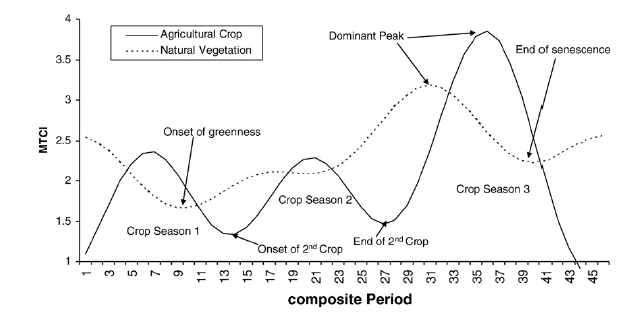
\includegraphics[width=\linewidth]{Images-phenology-fda/PhenoVars_Jegan.png} \isucaption{Diagram illustrating typical phenology patterns for agricultural land and natural vegetation from \cite{Dash:2010kva}. } \label{fig:phenology diagram} 
\end{figure}



\begin{figure}
	[htbp] 
	%\includegraphics[width=0.49\linewidth]{Images-phenology-fda/Satellite/India-current.png} 
	\hspace{1.5cm}\includegraphics[width=0.55\linewidth]{Images-phenology-fda/Satellite/India-5-12-2000.png}   \\
%	\includegraphics[width=\linewidth]{Images-phenology-fda/Satellite/southern_India_Google_Earth.png}   \\
	\includegraphics[width=\linewidth]{Images-phenology-fda/land_cover.pdf}
	 \isucaption{Google Earth\textsuperscript{TM} [data ISO, NOAA, U.S. Navy, NGA, GEBCO, Image Landsat] screenshot of study region in souther India from May 2000 (top). Land cover classification at 4.6~km spatial resolution derived from GLC2000 land cover database (bottom). } \label{fig:land cover} 
\end{figure}

\begin{figure}
	[htbp] \centering 
	\includegraphics[width=\linewidth]{Images-phenology-fda/mean_by_LC_facet_year.pdf} \isucaption{Smoothed MTCI values by year and by land cover.} \label{fig:mean by LC} 
\end{figure}

\begin{figure}
	[htbp] \centering 
	\includegraphics[width=\linewidth]{Images-phenology-fda/Plots/landcover_ag_veg.pdf} \isucaption{Land cover map of the study region aggregated into ``Agriculture'', ``Vegetation'', and ``other''. Grid cells were labeled ``Vegetation'' if their original land cover was Tropical Evergreen, Subtropical Evergreen, Tropical Semievergreen, Tropical Moist Deciduous, or Coastal vegetation. Grid cells were labeled ``Agriculture'' is their original land cover was Rainfed Agriculture, Slope Agriculture, Irrigated Agriculture, or Irrigated Intensive Agriculture. Black dots show the location of homogeneous agriculture grid cells.} \label{fig:land cover ag vs. veg} 
\end{figure}
\begin{figure}
	[htbp] \centering 
	\includegraphics[width=\linewidth]{Images-phenology-fda/Plots/proportion_agriculture.pdf} \isucaption{Map of the study region showing the proportion of agricultural land within each of the 4.6~km$\times$4.6~km grid cells based on the GLC2000 land cover database. } \label{fig:proportion agriculture} 
\end{figure}

% \begin{figure}
% 	[htbp] \centering
% 	\includegraphics[width=\linewidth]{Images-phenology-fda/ag_hom_cells.pdf} \isucaption{Map of the study region showing the location of homogeneous agriculture grid cells. } \label{fig:homogeneous ag cells}
% \end{figure}

\begin{figure}
	[htbp] \centering 
	\includegraphics[width=\linewidth]{Images-phenology-fda/hom_curves_agriculture_east_west_2003_2.pdf} \isucaption{Observed MCTI values for homogeneous agriculture cells in 2003. The color identified curves as either in the eastern or western part of the country. The homogeneous agriculture cells on the west side of the country consist of intensely irrigated agriculture. } \label{fig:ag cell east vs west} 
\end{figure}


% section data (end)
\section{Methodology} 
% (fold)
\label{sec:methodology}

The data have both a rich spatial and temporal component. We view the data as a collection of curves that are each a function of time, but have the attribute of a spatial location. The map in Figure \ref{fig:land cover} consists of many different land cover types largely separated on the east and west by agricultural land and natural vegetation, respectively. Our primary interest is to be able to detect locations that are possibly misclassified as natural vegetation. Our general approach consists of the following steps:
\begin{itemize}
	\item Label each cell as either vegetation, agriculture, or other. Figure \ref{fig:land cover ag vs. veg} shows the land cover map using this labeling.
	\item Construct a set of empirical basis functions derived from land that is primarily agricultural. We only include homogeneous agriculture cells defined to be cells with 100\% agricultural land cover according to the proportions derived from the GLC2000 database. Figure \ref{fig:proportion agriculture} shows the proportion of agricultural land based on GLC2000 database, and Figure \ref{fig:homogeneous ag cells} shows the location of the homogeneous agricultural cells. The homogeneous agriculture cells on the western side of the country are irrigation intensive agriculture and exhibit different phenological patterns than agriculture cells on the eastern part of the country as can be seen in Figure \ref{fig:ag cell east vs west}. For this reason we did not include these locations in the set of homogeneous agriculture locations. 
	\item Project all of the data onto the basis, reducing the information for each curve to a low dimensional vector of coefficients.
	\item Construct a classifier for the coefficient vectors by using a training set corresponding to the homogeneous agriculture locations and an equal number of homogeneous vegetation locations.  
\end{itemize}

\subsection{Functional model for homogeneous grid cells} % (fold)
\label{sub:subsection_name}

 For the set of homogeneous agricultural grid cells we model the phenological trajectories $X(t)$ as a continuos second order stochastic process with mean $\mu(t)$ and bivariate temporal covariance function
\[ C_{0}(s,t)=E([X(s)-E(X(s))][X(t)-E(X(t))]),\mbox{ }\forall s,t\in \T. \]
We analyze the process on an annual basis which for the 8-day composite MCTI values corresponds to the time domain $\T = [0,46]$, but in what follows the data are rescaled to the interval $[0,1]$. We assume the underling trajectories $X(\cdot)$ are smooth in that they take values in a reproducing kernel Hilbert space $\H= \{f : f, f' \mbox{ absolutely continuous}, f'' \in L_2[0,1]\}$. 

Let $\{X_{1},X_{2},\dots,X_{N}\}$ represent the collection of realizations of $X$, and we consider the following model for the observed MCTI values $Y_{ij}$,
\[ Y_{ij}=X_{i}(t_{ij})+\epsilon_{ij},\mbox{ }j=1,\dots,46;\mbox{ }i=1,\dots,N, \]
where $i$ indexes the centroid of the spatial grid cell and $j$ indexes the sampling times corresponding to the 8-day composite MTCI values. The $\epsilon_{ij}$ are independently and identically distributed measurement errors with mean zero and finite variance $\sigma_{0}^{2}.$ It is further assumed that the random functions $X$, and measurement errors $\epsilon$ are mutually independent. 
% subsection subsection_name (end)

\subsection{Smoothing} 

% (fold)
\label{sub:smoothing}
We achieve smooth versions of the observed curves by expressing them as a finite basis expansion of principal component functions corresponding the the covariance function $C_0(s,t)$. The covariance of the observed process $Y_{ij}$ is given by
\begin{equation}
	C(Y_i(t_j), Y_i(t_k)) = C_0(X_i(t_j), X_i(t_k)) + \sigma^2_0 \delta_{jk}
\end{equation}
where $\delta_{jk}$ equals 1 if $j=k$ and is equal to zero otherwise. The covariance function $C_0(s,t)$ is recovered by performing bivariate smoothing on the sample covariance omitting the diagonal values. The methodology, which is described in detail in described in Chapter \ref{ch:covariance estimation}, achieves both efficient estimation of $C_0(s,t)$ and results in closed-form estimates of corresponding principal component functions. For trajectories $X$ belonging to a reproducing kernel Hilbert space, optimal convergence properties are acheived due to the fact that the covariance function necessarily resides in the tensor product space $\H\tprod\H$. This fact motivates the following covariance function estimator.

Let $\mathbf{b}^{(i)} = [(Y_{ij}-\mu(t_{ij}))(Y_{ij'}-\mu(t_{ij'}))]_{1\leq j\neq j'\leq 46}$, $i=1, \dots, N$. Further, let
\[ \mathbf{b} = (\mathbf{b}^{(1)T}, \mathbf{b}^{(2)T}, \dots, \mathbf{b}^{(n)T} )^T, \]
where the vectors $\mathbf{b}^{(i)}$ contain all pairwise products of observations on the $i$th curve, excluding those that are the product of an observation with itself which correspond to the diagonal values on $[0,1]\times [0,1]$. Using this notation the covariance estimator corresponds to the following optimization problem,
\begin{equation}
	 \widehat{C}_{\lambda}=\stackrel[C \in \H\otimes \H]{}{\text{ argmin}} \left\{\frac{1}{n46^2-n46} (\mathbf{b} - \mathbf{C})^T(\mathbf{b} - \mathbf{C})+\lambda\left\Vert C\right\Vert _{\breve{\H}}^{2} \right\},
	 \label{pheno: cov est}
	 \end{equation}
where
\[ \mathbf{C} = [C(t_{i,j}, t_{i'j'})] \]
and $\lambda$ is a smoothing parameter estimated using cross validation.

In order to account for possible spatial correlation between curves we apply the weighting scheme developed in Chapter \ref{ch:functional kriging}. In Section \ref{sub:weighted covariance} we showed that we can achieve significant improvements in covariance estimation by down weighting curves corresponding to high location density areas.

We proceed to define location intensity as the number of locations per unit area and denote location intensity at location $i$ by $\gamma_i$.  The following weight function provides a simple yet flexible way to construct weights,
\begin{equation}
	w_i = \left(\frac{1}{\gamma_i}\right)^p. \label{pheno:weight function}
\end{equation}
The weight function \eqref{pheno:weight function} includes a scaling parameter, $p$, whose appropriate value depends on the degree of spatial dependence in the data. In the section \ref{sub:selecting_an_appropriate_weight} we describe how to investigate possible values for $p$.


Let $\mathbf{W} = diag(\mathbf{w}_1, \dots, \mathbf{w}_n)$, where $\mathbf{w}_i$ is a row vector whose length is equal to the length of $\mathbf{b}^{(i)}$ and whose components are all equal to $w_i$. The spatially re-weighted covariance estimator is constructed by replacing the loss function in \ref{pheno: cov est} with 
\begin{equation}
	l(C)= (\mathbf{b} - \mathbf{C})^T\mathbf{W}(\mathbf{b} - \mathbf{C}). \label{pheno:diag weighted loss function} 
\end{equation}
Details of the estimation of $\widehat{C(s,t)}$ and its corresponding eigenfunctions $\hat{\psi}_k(t)$ are described in Chapter \ref{ch:covariance estimation}. 

To produce smooth estimates of the trajectories $X_i(t)$, project the observations $Y_i(t_j), j = 1, \dots, 46$ onto the finite dimensional functional basis $\{\hat{\psi}_k(t), k = 1, \dots, q\}$, where $q$ is chosen such that at least $90\%$ of the variation is explained. The fitted trajectories admit the following representation
\begin{equation}
	\widehat{X_i(t)} = \sum_{k=1}^q\alpha_{k,i} \hat{\psi}_k(t) = \boldsymbol{\alpha_i'}\boldsymbol{\psi}.
	\label{phen:coef}
\end{equation}
In this representation the randomness associated with each random trajectory $X(t)$ is captured in the coefficient vector $\boldsymbol{\alpha}$. This allows one to take advantage the vast methods available for multivariate data. In this work we use linear discriminant analysis to classify land cover, but this framework allows for many possibilities for using multivariate methods for functional data analysis. 
\subsubsection{Selecting an appropriate weight} 

% (fold)
\label{sub:selecting_an_appropriate_weight} 
Selection of the weight parameter $p$ in \eqref{pheno:weight function} is a challenging problem as the optimal choice fundamentally depends on the strength of dependence in the data. However, simulations presented in Chapter \ref{ch:functional kriging} indicate that precision in estimating the value of $p$ is not necessary by observing that values between 1/3 and 1/2 are suitable for varying levels of spatial dependence. We performed a similar simulation study using the same framework, but using locations corresponding to the homogeneous agriculture grid cells. The simulation results using the homogeneous agriculture locations were consistent with the results in Chapter \ref{ch:functional kriging}. Based on these results we used $p=1/2$ to define the weights. The locations and their weights derived from \eqref{pheno:weight function} using $p=1/2$ are shown in Figure \ref{fig:india weighted locs}. 
\begin{figure}
	[h] \centering 
	\includegraphics[width=0.7\linewidth]{Images-phenology-fda/india_wt_locs.pdf} \isucaption{Spatial locations of the homogeneous agricultural grid cells. The size of the point indicates the weight used for data at that location for estimating the covariance function. } \label{fig:india weighted locs} 
\end{figure}


% subsection selecting_an_appropriate_weight (end)
% subsection smoothing (end)
\subsection{Land cover classification} 
 % (fold)
\label{sub:land_cover_classification}

The representation of each curve in terms of the FPC expansion \eqref{phen:coef} associates to each trajectory a set of $q$ coefficients. The dimension reduction achieved with this representation allows one to bring to bare any number of classical statistical methods---which is the major benefit of this approach. We describe a method for classification suitable for this type of data structure motivated by the phenological application as follows.

%We describe two methods for classification suitable for this type of data structure, one using linear discriminant analysis and one using logistic regression motivated by the phenological application as follows. 

\subsubsection{Linear Discriminant Analysis} % (fold)
\label{sub:LDA}
Linear discrimant analysis is a popular method in the class of linear classifiers; here the term linear referes to the structure of the decision boundary. Let $\mathcal{C} = \{ \text{Agriculture}, \text{Vegetation}\}$ be the set of all possible classes, and let C be a random variable taking values in $\mathcal{C}$. The classification decision is based on the rule
\begin{equation}
	\hat{\text{C}}(\boldsymbol{\alpha}) = 
	\begin{cases}
			\text{Agriculture} \hfill & \text{ if } \text{Pr}(\text{C = Agriculture }| \boldsymbol{\alpha})> \text{Pr}(\text{C = Vegetation }| \boldsymbol{\alpha})\\
			\text{Vegetation} \hfill & \text{ otherwise}
	\end{cases}
\end{equation}  
Computation of the posterior probabilities follows from modeling the class-conditional densities $f_k(\boldsymbol\alpha)$ as multivariate Gaussian distributions
\begin{equation}
	f_k(\boldsymbol\alpha) = \frac{1}{(2\pi)^{p/2}}e^{-\frac{1}{2}(\boldsymbol\alpha - \boldsymbol\mu_k)^T\Sigma^{-1}(\boldsymbol\alpha - \boldsymbol\mu_k)}
\end{equation}
and the assumption in LDA is a common covariance matrix between classes. With this assumption 
\begin{equation}
	\text{Pr}(\text{C} = \text{Agriculture } | \boldsymbol\alpha) = \frac{f_{ag}(\boldsymbol\alpha)\pi_{ag}}{f_{ag}(\boldsymbol\alpha)\pi_{ag}+f_{veg}(\boldsymbol\alpha)\pi_{veg}}
\end{equation}
where $\pi_{ag}$ and $\pi_{veg}$ are the prior probabilities class membership. Training data are used to estimate all parameters using maximum likelihood. The strong distributional assumptions make this approach computationally efficient, but diagnostics should be used to check if the assumption of multivariate Gaussian distributions with common covariance structure is reasonable. 
 % subsection LDA (end)

% \subsubsection{Logistic Regression} % (fold)
% \label{sub:subsection_name}
%
% % subsection subsection_name (end)
% The coefficient vectors are low dimensional and can be used effectively as covariates because colinearity is mitigated by the used of FPCs. We describe an approach for classification using a logistic regression model.
%
% Let $Z_i$ be a random variable connected to the land cover class of spatial grid cell location $i$, which takes values in $\{0,1\}$ corresponding the classes $\{$Vegetation, Agriculture$\}$. Logistic regression is a special case of a generalized linear model whose random component is modeled as a Bernoulli distribution and whose link function is logit(p),
% \begin{equation}
% 	Z_i | \alpha_{1,i}, \dots, \alpha_{4,i} \sim \text{Bernoulli}(p_i) \nonumber
% \end{equation}
% and
% \begin{equation}
% 	ln \left(\frac{p_i}{1-p_i}\right) = \beta_0 + \beta_1 \alpha_{1,i} + \dots + \beta_4 \alpha_{4,i}.\nonumber
% \end{equation}
% The fitted values $\hat{p_i} = \text{E}[Z_i| \alpha_{1,i}, \dots, \alpha_{4,i} ]$ are estimates of the probably that location $i$ has an agriculturally dominant land cover. The classifier we use follows the rule
% \begin{equation}
% 	\text{land cover}_i =
% 	\begin{cases}
% 			\text{Agriculture} \hfill & \text{ if $\hat{p}_i >= 1/2$}\\
% 			\text{Vegetation} \hfill & \text{ if $\hat{p}_i < 1/2$}
% 	\end{cases}
% 	\nonumber
% \end{equation}



% subsection land_cover_classification (end)
% section methodology (end)
\section{Results} 
% (fold)
For each year function principal components were computed and for all years only three FPCs were needed to account for at least 90\% of the variation based on the eigenvalues. The first three FPCs for each year are shown in Figure \ref{fig:pcf all years}. These functions and a constant function were used as basis functions which were fit to all locations. The classification results are shown in Figures \ref{fig:misclassified vegetation} and \ref{fig:misclassified agriculture}, where only discrepancies in classification between the classifier proposed in this work and the GLC2000 classification are shown with highlighted red cells. Figure \ref{fig:misclassified vegetation} indicates and extensive area in the northern part of the study region that is being classified as agriculture by the LDA classifier, but is labeled as natural vegetion using the GLC2000 data base. 

Figures \ref{partimat 2003}, \ref{partimat 2004},\ref{partimat 2005},\ref{partimat 2006}, and \ref{partimat 2007} show LDA estimates for all unique pairs of variables with colors highlighting the linear decision boundary. These Figures indicate that the model assumptions are not a concern in this case, and that a linear decision boundary is likely sufficient for these data. 

\begin{figure}
	[htbp] \centering 
	\includegraphics[width=\linewidth]{Images-phenology-fda/PCF_all_years.pdf} \isucaption{First three principal component functions computed for each year from 2003-2007. } \label{fig:pcf all years} 
\end{figure}

\begin{figure}
	[htbp] \centering 
	\includegraphics[width=\linewidth]{Images-phenology-fda/Plots/misclassified_vegetation.pdf} \isucaption{Map of the study region showing locations where classification results differ from the original GLC2000 derived land classification. Locations that the GLC2000 identified as vegetation, but were classified as agricultural are shown in red.   } 
	\label{fig:misclassified vegetation} 
\end{figure}

\begin{figure}
	[htbp] \centering 
	\includegraphics[width=\linewidth]{Images-phenology-fda/Plots/misclassified_agriculture.pdf} \isucaption{Map of the study region showing locations where classification results differ from the original GLC2000 derived land classification. Locations that the GLC2000 identified as agriculture, but were classified as natural vegetation are shown in red.} 
	\label{fig:misclassified agriculture} 
\end{figure}

\begin{figure}
	[htbp] \centering 
	\includegraphics[width=\linewidth]{Images-phenology-fda/Plots/prob_ag.pdf} \isucaption{ Posterior probability of Agricultural land cover. } 
	\label{fig:probability map} 
\end{figure}


\label{sec:results}


% section results (end)
\section{Conclusions} 
We have developed an approach to land cover classification between agricultural and natural vegetation using observe MTCI data. The classification maps shown in Figure \ref{fig:misclassified vegetation} indicate that a large number of locations that the GLC2000 based classification labelled as natural vegetation are being classified as agriculture. Many of the discrepancies are along the center ridge of where it is not surprising to see conflicting classifications as this is where the agricultural east converges with the tropical west; however there are two areas within on the west side of the country that seem to be consistently classified as agricultural: a large area toward the northern border of the region, and a small grouping of cells near the middle of the western side of the country. 

Satellite imagery sheds some light on what might be causing this effect. Figure \ref{fig:north india} shows a zoomed in satellite image of the northern area of the region both in the year 2000 and in 2003. There appears to be large area of possible deforested land that is much more apparent in 2003 than it is the satellite picture from 2000. Figure \ref{fig:north india zoom} shows a high resolution image of the deforested area. This finding shows that the classification method is effective at detecting anthropomorphic changes in vegetation land cover using the MTCI data. 

The map in Figure \ref{fig:proportion agriculture} shows the proportion of agricultural land in each grid cell based on the GLC2000 database. This map indicates that some cells in the two regions we have identified had some agricultural land cover according to the GLC2000 database, but not to the spatial extent that we observe in the MTCI classification. That is, many of the grid cells consistently classified as agriculture by the MTCI classification have near zero proportion of agricultural land according to the GLC2000 database. This suggests an actual change over time (since 2000) of land cover in these areas which could correspond to increased deforestation, increased agriculture development, or both. 

The results do not necessarily indicate an increase of agricultural land over time, as the classification is not completely consistent over time in many areas. For example, it is 2003 where the most vegetation land is classified as agriculture. This may indicate that mixed land cover cells exhibit the behavior of natural vegetation or agriculture depending on the year. The point, however, is not to say these cells \emph{are} agricultural or \emph{are} natural vegetation, but to recognize that they are neither and should be given careful consideration---and possibly omitted---for analyses that seek to characterize phenological variables with respect to land cover. 


% (fold)
\label{sec:discussion}


\begin{figure}
	[htbp] \centering 
%	\includegraphics[width=0.7\linewidth]{Images-phenology-fda/Plots/landcover_overlay_background.png} \\[0.5cm]
	\includegraphics[width=\linewidth]{Images-phenology-fda/Plots/landcover_overlay.png} \\
	\isucaption{Google Earth\textsuperscript{TM} [data ISO, NOAA, U.S. Navy, NGA, GEBCO, Image Landsat] image of northwestern part of the study region in southern India in 2014 (top). Areas in the year 2007 designated as agricultural by the LDA classifier, but labeled as vegetation by the GLC2000 database are shown in red (bottom).} 
	\label{fig:classification overlay} 
\end{figure}

\begin{figure}
	[htbp] \centering 
	\includegraphics[width=0.7\linewidth]{Images-phenology-fda/Satellite/India-2000.png} \\[1cm]
	\includegraphics[width=0.7\linewidth]{Images-phenology-fda/Satellite/India-10-10-2003.png} \\
	\isucaption{Google Earth\textsuperscript{TM} [data ISO, NOAA, U.S. Navy, NGA, GEBCO, Image Landsat] image of northwestern part of the study region in southern India from 2000 (top) and 2003 (bottom). } 
	\label{fig:north india} 
\end{figure}

\begin{figure}
	[htbp] \centering 
	\includegraphics[width=0.7\linewidth]{Images-phenology-fda/Satellite/India-12-29-2003.png} \isucaption{Google Earth\textsuperscript{TM} [data ISO, NOAA, U.S. Navy, NGA, GEBCO, Image Landsat] image of study region in souther India showing an area of possible deforestation and agricultural development.} 
	\label{fig:north india zoom} 
\end{figure}
% section conclusion (end)

\section{Supplementary material} % (fold)
\label{sec:supplementary_material}

\begin{figure}
	[htbp] \centering 
	\includegraphics[width=0.8\linewidth]{Images-phenology-fda/Plots/partimat_2003.pdf}  \isucaption{Plot of linear discriminant analysis decision boundary for all 2-d partitions the empirical basis functions using data from 2003.}
	\label{partimat 2003} 
\end{figure}
\begin{figure}
	[htbp] \centering 
	\includegraphics[width=0.8\linewidth]{Images-phenology-fda/Plots/partimat_2004.pdf}  \isucaption{Plot of linear discriminant analysis decision boundary for all 2-d partitions the empirical basis functions using data from 2004.}
	\label{partimat 2004} 
\end{figure}
\begin{figure}
	[htbp] \centering 
	\includegraphics[width=0.8\linewidth]{Images-phenology-fda/Plots/partimat_2005.pdf}  \isucaption{Plot of linear discriminant analysis decision boundary for all 2-d partitions the empirical basis functions using data from 2005.}
	\label{partimat 2005} 
\end{figure}
\begin{figure}
	[htbp] \centering 
	\includegraphics[width=0.8\linewidth]{Images-phenology-fda/Plots/partimat_2006.pdf}  \isucaption{Plot of linear discriminant analysis decision boundary for all 2-d partitions the empirical basis functions using data from 2006.}
	\label{partimat 2006} 
\end{figure}
\begin{figure}
	[htbp] \centering 
	\includegraphics[width=0.8\linewidth]{Images-phenology-fda/Plots/partimat_2007.pdf}  \isucaption{Plot of linear discriminant analysis decision boundary for all 2-d partitions the empirical basis functions using data from 2007.}
	\label{partimat 2007} 
\end{figure}

% section supplementary_material (end)





%%% Appendix %%%
%%!TEX root = ../dissertation.tex
\appendixtitle
\appendix
\chapter{Theoretical background on smoothing splines and reproducing kernel Hilbert space}
 \label{ch:theoretical background}


\section{Historical note on the use of reproducing kernel Hilbert spaces in statistics}

This section contains some historical context to understand the motivation for the mathematical framework of reproducing kernel Hilber space and their use in statistics. In the following I would like to describe a little bit about how these special Hilbert spaces became mainstream in statistics and mention some of the key players. 
%\begin{figure}[h] %  figure placement: here, top, bottom, or page
%   \centering
%      \begin{subfigure}[b]{0.40\textwidth}
%                \centering
%                \includegraphics[width=.5\textwidth]{Images-general-introduction/parzen.pdf}
%                %\caption{Emanuel Parzen}
%                \label{}
%        \end{subfigure}%
%        \begin{subfigure}[b]{0.40\textwidth}
%                \centering
%                \includegraphics[width=.5\textwidth]{Images-general-introduction/wahba.pdf}
%                %\caption{Grace Wahba}
%                \label{}
%        \end{subfigure}
%   \caption{Emanuel Parzen and Grace Wahba}
%   \label{fig:example}
%\end{figure}


The origin of reproducing kernel Hilbert space methods in statistics is due to Emanuel Parzen. In an interview in a 2002 issue of Statistical Science, Parzen describes how he was introduced to the topic. He states that when he was a graduate student at Berkely, students did not take the usual Ph.D qualifying exam; instead, each student was tasked with giving a lecture to their committee on a specific topic --- Parzen's topic: reproducing kernels. When he began studying the topic, he only found one source in the literature and it was in French. The paper he found was work by Aronszajn, who had developed the abstract theory of reproducing kernels to generalize kernel methods popular in applied mathematics. 

The use of Hilbert space methods to model continuous-parameter time series appears to be the Parzen's initial application of reproducing kernels in statistics. Though Parzen was working on time series analysis, it seems that the reproducing kernel framework is used more widely in the smoothing spline methods as a regularization approach for nonparametric curve estimation due to the fact that minimization problems over a RKHS have a unique solution with a finite dimensional representation (the so-caledl representer theorem). It was Parzen's graduate student Grace Wahba who championed regularization via RKHS in her book, \emph{Spline Models for Observational Data} (\cite{Wahba:1990}). Most of the current work using a RKHS framework for nonparametric estimation cite Wahba�s work, and it is telling that a lot of the current researchers on smoothing spline methods are themselves former students of Grace Wahba (e.g. Chong Gu, Yuedong Wang, Ming Yuan, Doug Nychka). In the introduction to her book, Grace Wahba offers some encouragement, which I have included below in quotations. I took this advice to heart when I first embarked on this topic --- I have to say that she has been true to her word. 
\begin{quote}
``I would like to assure the reader that the effort to master the basic properties of reproducing kernel Hilbert spaces, will be worth the effort.''\\
-Grace Wahba
\end{quote}

\section{ Going beyond ordinary least squares: Penalized least squares and the cubic smoothing spline} 


\subsection{Least Squares Estimation}
Consider the regression problem where observations $(x_i, y_i), i=1,\dots,n,$ are modeled as $y_i = f(x_i) + \epsilon_i, \epsilon_i \sim N(0,\sigma^2).$ This model assumes that we observe an underlying signal, $f$, corrupted by noise. The desire is to recover $f$ from the observations $(x_i, y_i), i=1,\dots,n$. The noise terms $\{\epsilon_i\}$ are random variables and exact recovery of $f$ is not possible, thus our goal becomes to find a good approximation to $f$. The least squares estimator of $f$ is given by the minimizer $\hat{f}$ of the sum of the squared deviations over all functions $f \in \mathcal{A}$ 
\begin{equation*}
\hat{f} = \hspace{.07in} \stackrel[f \in \mathcal{A}]{}{\mbox{argmin}} \frac{1}{n}\sum_{i=1}^{n}(y_i - f(x_i))^2.
\label{eq:LS}
\end{equation*}

If the underlying signal $f$ does not lie in $\A$, then the estimator is guaranteed to be biased. In order to avoid misspecification of $\A$, a wide class of functions should be considered.  As a concrete example, in simple linear regression we have $\A = \{f: f(x_i) = \beta_0 + \beta_1x_i ; i=1,\dots,n \}$. In this setting, $\A$ is defined as the two dimensional subspace of $\Real^n$ spanned by a column of 1s and the column vector $(x_1,\dots, x_n)'$. The matrix consisting of these columns constitutes the \textit{model matrix.} Any function $f \in \A$ can be identified uniquely by the parameters $\beta_0$ and $\beta_1$ in its representation as a linear combination of the columns of the model matrix. Thus, the solution to the least squares minimization problem has the representation $\wh{f} = X\wh{\bbeta}$ satisfying 
\begin{equation*}
\widehat{\bbeta} =  \hspace{.07in}  \stackrel[\bbeta \in \Real^2]{}{\mbox{argmin}} (\textbf{Y} - \textbf{X}\bbeta)'(\textbf{Y} - \textbf{X}\bbeta)
\label{eq:LS2}
\end{equation*}
where $\textbf{Y}=(y_1,\dots, y_n)'$, and $\textbf{X}$ is the model matrix. Finding $\widehat{\bbeta}$ requires simple matrix calculus manipulations. 

\subsection{Penalized Least Squares} \label{PLS}
  The purpose of presenting the simple linear regression problem in the previous section was to emphasize how the choice of a parametric model can be framed as a choice of the structure of the function space $\A$. The simple linear regression model is equivalent to specifying $\A$ to be a known 2-dimensional subspace of $\Real^n$ -- the column space of $\textbf{X}$. In practice, many relationships of interest are approximately linear making this model suitable in such cases. However, in most applications it is not the \textit{truth} of the model we believe in, but its adequacy as a mathematical representation of the underlying relationship. When a parametric model is adequate the parameters often give us insight into the structure of the relationship and scientific questions of interest can often be stated in using contrasts of the parameters. However, there is usually very little known about the functional form of $f$, and hence there is very little justification for restricting the estimator to belong to a particular class of parametric functions. 
 
Therefore, it seems desirable to consider a larger class of functions. To decide on how large this class should be, we remark that any reasonably large class of functions will contain functions that interpolate the data. Since we believe the observational process is corrupted by noise, we do not wish to model the idiosyncrasies of the data; that is,  we believe the estimator $\hat{f}$ must be smoother than an interpolating function. Penalized least squares is one method where this problem is addressed by including a term that penalizes the roughness of the function. The penalized least squares estimator of $f$ is formulated to balance two competing functionals 
\begin{equation}
\widehat{f}_{\lambda} = \hspace{.07in}\stackrel[f \in \A]{}{\mbox{argmin}} \left\{ \frac{1}{n}\sum_{i=1}^{n}(y_i - f(x_i))^2 + \lambda\int_{\X}(f''(x))^2dx \right\},
\label{eq:PLS}
\end{equation}
where the smoothing parameter $\lambda$ governs the trade-off between fitting the data and smoothness of the function. In \eqref{eq:PLS} the smoothness of the function is measured by the integral of its squared second derivative, thus implicitly assuming the second derivative exists and that it is square integrable. A natural functional space to consider is the space $\A = \{f: f, f' \mbox{are absolutely continuous and } \int_0^1f''(x)^2dx <\infty\}$. It is important to note that linear functions are not penalized in \eqref{eq:PLS} and as $\lambda \rightarrow \infty$ the estimator $\wh{f_{\lambda}}$ converges to the least squares estimator. Two important questions to consider are: 
\begin{enumerate}
	\item Is there a solution to the minimization problem in \eqref{eq:PLS}?
	\item Is the solution unique?
\end{enumerate}
The answer is affirmative to both questions; furthermore, the solution is a piecewise cubic polynomial.  To better understand how to solve minimization problems like \eqref{eq:PLS} we consider the Hilbert space structure of $\A$, and show how the existence of a reproducing kernel is key. 
 

%============================================================================================================================
\section{Reproducing kernel Hilbert spaces (RKHS)}
%============================================================================================================================

%=======================================================================================================
\subsection{Notation and basic definitions}


In this section we will cover a brief introduction to reproducing kernel Hilbert spaces. Two excellent introductions to this material are given in \cite{Heckman:1997vp} and \cite{Storlie:2011tz}, while more rigorous presentations are given by \cite{Wahba:1990} and \cite{Aronszajn:1950tq}. 
Notice that in \eqref{eq:PLS} the sum of squares term involves evaluation of $f$. A reproducing kernel Hilbert space is a Hilbert space where function evaluation is a continuous linear operator. That is a Hilbert space $\H$ on a domain $\T$ is a reproducing kernel Hilbert space if $L_t(f) = f(t)$ is continuous in $\H$, $\forall t \in \T$. The domain $\T$ often represents a continuous time domain and will typically be the close interval $[0,1]$. It is well known that continuity of a linear functional is equivalent to boundedness of the functional, where boundedness means that there exists an $M_t$ such that 
\begin{equation*}
	|L_t(f)|=|f(t)|\leq M_t\norm{f}_{\H}, \mbox{ for all $f$ in the RKHS}.
\label{eq:}
\end{equation*}
The Riesz representation theorem states that any continuous linear operator on $\H$ has a representation in terms of the inner product on $\H$
\begin{equation}
	L_t(f) = \inner{R_t(\cdot)}{f(\cdot)} = f(t), \forall f\in \mathcal{H},
\label{eq:Riesz}
\end{equation}
where $R_t$ is a function in $\H$. If we denote $R_t(s)$ by $R(s,t)$, then the reproducing property in \eqref{eq:Riesz} implies that $\inner{R_s(\cdot)}{ R_t(\cdot)} = R(s,t)$. Note the $R(s,t)$ is a symmetric bivariate function defined on $\T\times\T$. %We will denote by $\H$$_R$ a RKHS with reproducing kernel R, and its inner product by $\langle\cdot,\cdot>_R$. 

At this point, we note that this reproducing property may appear to be similar to the use of the Dirac delta function $\delta$, where $f(x)=\int\delta(x-y)f(y)dy$. The key distinction is that $\delta$ is not an element of $\H$, in fact, $\delta$ is not even a function in the conventional sense.  As a concrete example the space $\L^2[0,1]$ is not a RKHS. To see this, consider the sequence of polynomials $f_n = x^n$ which converge to the null function, since $\norm{f_n-0}_2=(2n+1)^{-1/2}$, yet $f_n(1)=1$ for all $n$; i.e. $L_1(t)$ is not a continuous functional. It is easy to show that in RKHS, norm convergence implies pointwise convergence. 

The following result (Theoreom 2.5 in \cite{Gu2002}) will be useful in solving penalized least squares problems, where it is natural to consider a direct sum decomposition of the null space of the penalty term and its orthogonal complement. 
\begin{thm} \label{RKHS_decomposition}
If the reproducing kernel R of a space $\H$ on domain $\T$ can be decomposed into $R= R_0 + R_1$, where $R_0$ and $R_1$ are both non-negative definite, $R_0(x,\cdot), R_1(x,\cdot) \in \H, \forall t \in \T$, and $\inner{R_0(s,\cdot)}{R_1(t, \cdot)} =0, \forall s,t \in \T$, then the spaces $\H_0$ and $\H_1$ corresponding respectively to $R_0$ and $R_1$ form a tensor sum decomposition of $\H$. Conversely, if $R_0$ and $R_1$ are both non-negative definite and $\H_0 \cap \H_1 = {0}$, then $\H = \H_0 \oplus \H_1$ has a reproducing kernel $R = R_0 + R_1$. 
\end{thm}



%=============================================================================================================================
\subsection{Motivation for the use of RKHS in penalized regression} \label{motivation for RKHS}

In Section \ref{PLS} the space $\A = \{f: f, f' \mbox{are absolutely continuous and } \int_0^1f''(x)^2dx <\infty\}$ was chosen as a solution space for the optimization problem in \eqref{eq:PLS}. This space with the inner product $\inner{f}{g} = f(0)g(0) + f'(0)g'(0) + \int_0^1 f''(x)g''(x)dx$ is a Hilbert space with the reproducing property. In this section we derive the solution to \eqref{eq:PLS} highlighting the use of the reproducing property.  

Let $\H$ be a the Hilbert space $\{f: f, f' \mbox{are absolutely continuous and } \int_0^1f''(x)^2dx <\infty\}$ with inner product $\inner{f}{g} = f(0)g(0) + f'(0)g'(0) + \int_0^1 f''(x)g''(x)dx$. Notice that the penalty functional in \eqref{eq:PLS}, $\int_0^1f''(x)^2dx$, corresponds to a squared semi-norm with null space $\N = \{f: f=\alpha_0 + \alpha_1x\}$. This is a closed linear subspace of $\H$ which means $\H$ has a direct sum decomposition $\H = \H_0 \oplus \H_1$, where $\H_0 = \N$ and $\H_1 = \N^{\bot}= \{f: f(0)=f'(0)=0 \mbox{ and } \int_0^1(f''(x))^2dx < \infty\}$. Any $f \in \H$ has the representation $f = f_0 + f_1$, where $f_0 \in \H_0$ and $f_1 \in \H_1$. On $\H_1$ the penalty term $\int_0^1f''(x)^2dx$ corresponds to a full squared norm, thus the penalty term can be written as $\norm{P_1(f)}_{\H_1}^2$ where $P_1(f) = f_1$ is the projection of $f$ onto $\H_1$. This allows \eqref{eq:PLS} to be put in the more general form
\begin{equation*}
\widehat{f}_{\lambda} = \hspace{.07in}\stackrel[f \in \H]{}{\mbox{arg min}} \left\{ \frac{1}{n}\sum_{i=1}^{n}(y_i - f(x_i))^2 + \lambda\norm{P_1(f)}^2_{\H_1} \right\}.
\label{eq:PLS_norm}
\end{equation*}

Recall that in the discussion of the least squares estimation problem in Section \ref{PLS} the minimization problem was reduced to a matrix calculus problem by restricting the solution space to a finite dimensional space spanned by the columns of the model matrix. In the current problem the minimizer lies in a finite dimensional subspace---this is a direct consequence of the reproducing property. To see this, let us further decompose $\H_1$ into two orthogonal subspaces $\H_1 =\mbox{span}\{R_1(\cdot,x_i); i = 1,\dots, n\}$ and $\H_1\ominus \mbox{span}\{R_1(\cdot,x_i); i = 1,\dots, n\}$. Any function $f \in  \H$  has the representation 
\begin{equation*}
f(x) = \alpha_0 + \alpha_1x + \sum_{i=1}^n \beta_iR_1(x, x_i) + \eta(x)=f_0 + f_{1} + \eta.
\label{eq:ds_representation} %direct sum representation
\end{equation*}
Substituting this representation into \eqref{eq:PLS_norm} we have 

\begin{align}
\widehat{f}_{\lambda} &= \hspace{.07in}\stackrel[f \in \H]{}{\mbox{arg min}} 
\left\{ \frac{1}{n}\sum_{i=1}^{n}(y_i - \alpha_0 - \alpha_1x_i - \sum_{i=1}^n \beta_iR_1(\cdot, x_i) - \eta(x_i))^2 \right. \nonumber \\
	 & \mbox{\hspace{1.5in}} + \left. \lambda\norm{\sum_{i=1}^n \beta_iR_1(\cdot, x_i) + \eta}^2_{\H_1} \right\} \nonumber \\
	 & = \hspace{.07in}\stackrel[f \in \H]{}{\mbox{arg min}} \left\{ \frac{1}{n}\sum_{i=1}^{n}(y_i - \alpha_0 - \alpha_1x_i - \sum_{i=1}^n \beta_iR_1(\cdot, x_i) - \eta(x_i))^2 \right. \nonumber \\
  & \mbox{\hspace{1.5in}} + \left. \lambda\norm{\sum_{i=1}^n \beta_iR_1(\cdot, x_i) }^2_{\H_1} + \lambda\norm{\eta}^2_{\H_1} \right\}.
\label{eq:PLS_norm2}
\end{align}

The reproducing property allows us to express the function evaluation terms $\eta(x_i); i = 1,\dots, n$ as inner products with the reproducing kernel on $\H_1$
\begin{equation*}
\eta(x_i) = \inner{R_1(x_i,\cdot)}{\eta}; \hspace{0.1in} i = 1,\dots,n,
\label{eq:rep_property}
\end{equation*}
which is equal to zero for $i=1,\dots,n$ due to orthogonality. Thus, with this construction, $\eta$ only contributes to the minimization term through its norm, which is clearly minimized for $\eta$ equal to the zero function.

We now see that for a Hilbert space $\H$ where function evaluation is a continuous linear operator, the minimizer of \eqref{eq:PLS_norm2} has the form 
\begin{equation}
\widehat{f}_{\lambda} = \alpha_0 + \alpha_1x_1 + \sum_{i=1}^n \beta_iR_1(\cdot, x_i).
\label{eq:solution_form}
\end{equation}

In summary, we started with a minimization problem involving a smoothing penalty over a Hilbert space $\H$ and approached the problem by decomposing the space into orthogonal subspaces. The space $\H_0$ is the null space of the penalty term and defines the parametric contrasts; while the space $\H_1$ defines the non-parametric contrasts. If $\H$ is a RKHS, then the problem is simplified by only having to consider a finite dimensional subspace of $\H_1$. This simplification came from recognizing that point evaluation in the least squares functional could be re-expressed in terms of an inner product involving the reproducing kernel on $\H_1$, thus by choosing a subspace spanned by slices of the reproducing kernel on $\H_1$, the function $\eta$ no longer contributes to the least squares functional. The geometry of the Hilbert space, namely orthogonality, plays a critical role in this type of result and it is precisely continuity of the evaluation functional which allows point evaluation to be cast in terms of the geometry of the space.
%
%%==========================================================
%\section{Hilbert spaces generated by a non-negative definite kernel}
%%==========================================================
%
%Let $R:\T\times \T\rightarrow \Real$ by a symmetric non-negative definite
%kernel function. From Mercer's theorem $R(s,t)$ has the representation
%
%\[R(s,t)=\sum_{i=0}^{\infty}\gamma_{i}\phi_{i}(s)\phi_{i}(t)\]
%
%where the $\phi_{i}$ are eigenfunctions of the kernel function $R$
%corresponding to eigenvalues $\gamma_{i}$.
%Our interest in the space $\H_{R}\subset L^{2}(\T)$ with members
%\[
%f(t)=\sum_{i=1}^{\infty}c_{i}\phi_{i}(t)\] 
% for $c_{i} \mbox{ with  } \sum_{i=1}^{\infty}\frac{{c_{i}^{2}}}{\gamma_{i}}<\infty$ called the ``primal form'' of functions in the space. More naturally our interest centers on
%\[f(t)=\sum_{i=1}^{m}b_{i}R(s,t_{i})\] 
%for some set of $t_{i}$.
%
%Notice that 
%
%\[
%R(s,t)=\sum_{i=1}^{\infty}(\gamma_{i}\phi_{i}(s))\phi_{i}(t)=\sum_{i=1}^{\infty}c_{i}(s)\phi_{i}(t).
%\]
%Since \[\sum_{i=1}^{\infty}\frac{{c_{i}^{2}(t)}}{\gamma_{i}}=\sum_{i=1}^{\infty}\gamma_{i}\phi_{i}^{2}(t)= R(t,t)<\infty,\]
%the function $R(\cdot,t)$ belongs to the space. We define an inner product on the space by
%\[
%\left<\sum c_{i}\phi_{i},\sum d_{i}\phi_{i}\right>_{\H_{R}}\equiv\sum_{i=1}^{\infty}\frac{c_{i}d_{i}}{\gamma_{i}}.
%\]
%Note that for $f=\sum_{i=1}^{\infty}c_{i}\phi_{i}$, belonging to $\H_{R}$
%\[
%\left<f,R(\cdot,t)\right>=\sum_{i=1}^{\infty}\frac{{c_{i}\gamma_{i}\phi_{i}(t)}}{\gamma_{i}}=\sum_{i=1}^{\infty}c_{i}\phi_{i}(t)=f(t)
%\]
%and so $R(\cdot,t)$ is the representer of evaluation at $t$.
%
%Notice that reproducing property implies that for $f(t)=\sum_{i=1}^{m}b_{i}R(s,t_{i})$
%for some set of $t_{i},$
%\[
%\norm{f}_{\H_{R}}^{2}=<f,f>_{\H_{R}}=\sum_{i=1}^{m}\sum_{j=1}^{m}b_{i}b_{j}R(t_{i},t_{j})
%\]
%The optimization criterion 
%\[
%\frac{1}{n}\sum_{i=1}^{n}(y_{i}-f(t_{i}))+\lambda\norm{ f}_{\H_{R}}^{2}
%\]
%has, for training vectors $\{t_{i}\},$ the following representation
%\[
%\hat{f}(t)=\sum_{i=1}^{n}b_{i}R(t,t_{i})
%\]
%Thus the optimization reduces to minimizing, over choices of vectors $b$, the
%following
%\[
%(Y-\Rmat b)'(Y-\Rmat b)+\lambda b'\Rmat b.
%\]


%
%In applications, the positive definite kernel function must be specified. The following example from \cite{CFZ} hints at a procedure. In the solution to the cubic smoothing spline we derived a simple form of a positive definite kernel function
%\begin{equation}
%R(s,t) = 1 + st + \sum_{k=1}^{n}(s-t_k)_+(t-t_k)_+.
%\label{eq:simple_rk}
%\end{equation} 
%One can verify that the eigenfunctions associated with $R$ are
%\[
%\phi_0(t) =1, \phi_1(t)=t, \phi_{k+1}(t)=(t-t_k)_+ \mbox{   } k= 1,\dots,m-1,
%\]
%and the associate RKHS is
%\begin{equation}
%\H_R = \left\{ f:f(t) = \alpha_0 + \alpha_1t + \sum_1^n\beta_k(t-t_k)_+ \right\}
%\label{eq:css_space}
%\end{equation}
%with corresponding inner product
%\begin{align}
%<f,g>_{\H_R} &= \left<  \alpha_0 + \alpha_1t + \sum_1^n{\beta_k(t-t_k)_+}, \alpha'_0 + \alpha'_1t + \sum_1^n{\beta'_k(t-t_k)_+} \right>\\
%&= \alpha_0\alpha'_0 + \alpha_1\alpha'_1 + \sum_{k=1}^{n}{\beta_k \beta'_k}
%\label{eq:css_inner_prod}
%\end{align}
%From the definition of the inner product on the RKHS space with the chosen kernel we see that 
%\begin{equation}
%\norm{f}^2_{\H_R} = \norm{\alpha}^2 + \norm{\beta}^2.
%\label{eq:simple_norm}
%\end{equation}
%In practice it is often desired that some of the functions in $\H_R$ be unpenalized. In the case of penalized least squares the subspace of unpenalized functions is given by the null space of the differential operator which define $\H_0$. Therefore, functions $f \in \H_R$ are only penalized through their contribution in the subspace orthogonal to $\H_0$. In other words, only the projection of $f$ onto the space $\H_1$ is penalized. If $P_1f$ denotes the linear projection operator corresponding to the projection onto $\H_1$, then $\H_0$ is the null space of $P1$ and the solution has the form
%\begin{equation}
%\hat{f}_{\lambda} = \stackrel[f \in \H_R]{}{\mbox{arg min}}\left\{  L(f) + \lambda\norm{P_1f}^2_{\H_R} \right\}.
%\label{eq:penalized_solution}
%\end{equation}
%
%To summarize, even though \ref{eq:simple_rk} is the reproducing kernel on $\C^2[0,1]$ the solution to the cubic smoothing spline is not 
%\begin{equation}
%\hat{f}_{\lambda} = \stackrel[f \in \H_R]{}{\mbox{arg min}}\left\{  L(f) + \lambda\norm{f}^2_{\H_R} \right\}
%\label{eq:sol1}
%\end{equation} 
%The solution is given by \eqref{penalized_solution} due to the fact that linear functions are not penalized. The minimizer in \eqref{eq:sol1} has the representation $\sum_{k=1}^n\beta_k R(\cdot, t_k)$, whereas the minimizer in \eqref{eq:penalized_solution} has the representation $\sum_{i=1}^m \alpha_i\phi_i(t) + \sum_{k=1}^n\beta_k R_1(\cdot, t_k)$, where the $\phi_i$ are a basis for the null space of $P_1$ and $R_1$ is the reproducing kernel on $\H_1$. %Thus the minimizers in \eqref{eq:penalized_solution} and \eqref{eq:sol1} will not be the same unless $\norm{hat{f}_lambda} = \norm{P_1 \hat{f}_lambda}$, which will only be the case if $hat{f}_lambda$ has no linear component.

%%==========================================================
%\section{Tensor product reproducing kernel Hilbert spaces }
%%==========================================================

%%==========================================================
%\section{Tensor product smoothing splines on $[0,1]\times[0,1]$}
%%==========================================================
%
%
%\begin{thm}
%(Theorem 2.6 in Gu): For $R_{<1>}(x_{<1>}, y_{<1>})$ non-negative definite on $X_1$ and $R_{<2>}(x_{<2>}, y_{<2>})$ non-negative definite on $X_2$, $R(x,y) = R_{<1>}(x_{<1>}, y_{<1>})R_{<2>}(x_{<2>}, y_{<2>})$ is non-negative definite on $X = X_1 \times X_2$. 
%\end{thm}
%The RKHS corresponding to such an $R$ is called the tensor product space of $H_{<1>}$ and $H_{<2>}$, and is denoted by $H_{<1>}\otimes H_{<2>}$.  If each marginal domain is equipped with the decomposition in (\ref{eq:cubic_decomp}) then the tensor product space consists of 9 tensor sums. All of the tensor sums and their corresponding reproducing kernels are listed in Table \ref{tab:tp_decomp}. The subspace $H_{00<1>} \otimes H_{00<2>}$ spans the constant term, the subspaces $H_{00<1>}\otimes(H_{01<2>}\oplus H_{1<2>})$ and $(H_{01<1>}\oplus H_{1<1>})\otimes H_{00<2>}$ span the main effects, and the subspace $(H_{01<1>}\oplus H_{1<1>})\otimes(H_{01<2>}\oplus H_{1<2>})$ spans the interaction.
%
%
%
%\begin{table}[h]
%\begin{tabular}{|c|c|}
%\hline 
%Subspace & Reproducing Kernel\tabularnewline
%\hline
%\hline 
%$H_{00<1>}\otimes H_{00<2>}$ & 1\tabularnewline
%\hline 
%$H_{00<1>}\otimes H_{01<2>}$ & $k_{1}(x_{<2>})k_{1}(y_{<2>})$\tabularnewline
%\hline 
%$H_{00<1>}\otimes H_{1<2>}$ & $k_2(x_{<2>})k_2(y_{<2>}) - k_4(x_{<2>} - y_{<2>})$\tabularnewline
%\hline 
%$H_{01<1>}\otimes H_{00<2>}$ & $k_1(x_{<1>})k_1(y_{<1>})$ \tabularnewline
%\hline 
%$H_{01<1>}\otimes H_{01<2>}$ & $k_1(x_{<1>})k_1(y_{<1>})k_1(x_{<2>})k_1(y_{<2>})$ \tabularnewline
%\hline 
%$H_{01<1>}\otimes H_{1<2>}$ & $k_1(x_{<1>})k_1(y_{<1>})[k_2(x_{<2>})k_2(y_{<2>}) - k_4(x_{<2>} - y_{<2>})]$\tabularnewline
%\hline 
%$H_{1<1>}\otimes H_{00<2>}$ & $k_2(x_{<1>})k_2(y_{<1>}) - k_4(x_{<1>} - y_{<1>})$\tabularnewline
%\hline 
%$H_{1<1>}\otimes H_{01<2>}$ & $[k_2(x_{<1>})k_2(y_{<1>}) - k_4(x_{<1>} - y_{<1>})]k_1(x_{<1>})k_1(y_{<1>})$\tabularnewline
%\hline 
%$H_{1<1>}\otimes H_{1<2>}$ & $[k_2(x_{<1>})k_2(y_{<1>}) - k_4(x_{<1>} - y_{<1>})][k_2(x_{<2>})k_2(y_{<2>}) - k_4(x_{<2>} - y_{<2>})]$\tabularnewline
%\hline
%\end{tabular}
%\caption{Cubic smoothing spline tensor product space decomposition with corresponding reproducing kernels.}
%\label{tab:tp_decomp}
%\end{table}


%%!TEX root = dissertation.tex

\appendixtitle
\appendix
\chapter{ ssfcov2 package documentation} 

\includepdf[pages={1,2,3,4,5}]{Images-nonparametric/ssfcov2-manual.pdf}
%%% Bibliography %%%
\renewcommand{\bibname}{\centerline{BIBLIOGRAPHY}}
\unappendixtitle
\newpage
\phantomsection
\addcontentsline{toc}{chapter}{BIBLIOGRAPHY}
\bibliography{bib-dissertationnew.bib,books.bib}

%\listoftodos
\end{document} 
